\mathversion{sans}

\DeclarePairedDelimiter{\ivl}{[\mspace{-4.5mu}(}{)\mspace{-4.5mu}]}

\section{Introduction}

To maintain generality, the preceeding chapter leaves out some details; in particular, how to
\begin{enumerate}
	\item Represent and compute with abstract sets.
	\item Compute approximate preimages under real functions.
	\item Use preimage refinement to compute conditional probabilities efficiently.
\end{enumerate}
Figure~\ref{fig:implementation-components} puts these in a dependency graph in which nodes are modules in an implementation.
The boxes with dotted outlines are the subject of this chapter.

\begin{figure*}[b!]\centering
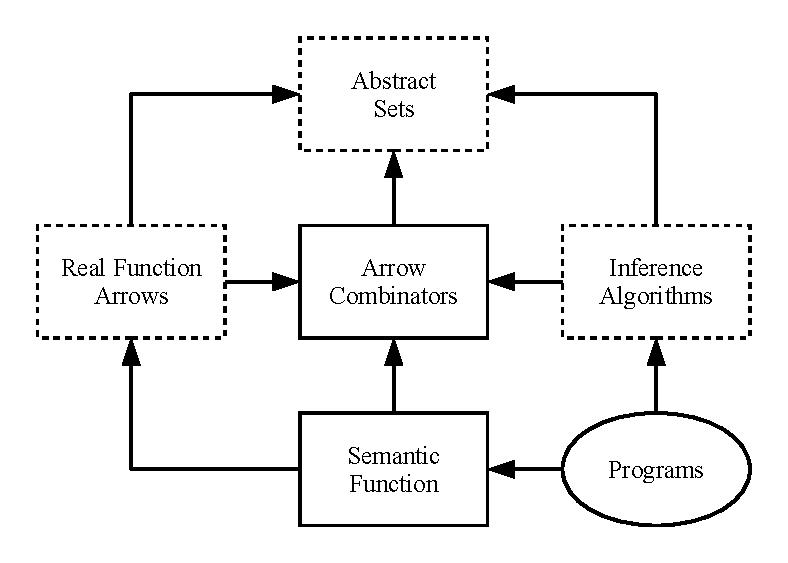
\includegraphics[width=4.75in]{figures/implementation-components}
\caption[Implementation dependency graph]{The components in an implementation, with dependence represented by arrows.}
\label{fig:implementation-components}
\end{figure*}

\section{Abstract Sets and Concrete Values}

While any kind of abstract sets with finite representations and computable operations would do, we use rectangles for their efficiency and simplicity, especially emptiness checking.

In a host language such as Haskell with sufficiently advanced typeclasses or an equivalent, it is possible to use polymorphism to represent rectangles in an extensible way.
For each required value type $X$, we need to define, in the host language,
\begin{itemize}
	\item A type of rectangles of $X$ with an associated type of members of $X$.
	\item Representations of the sets $\emptyset$ and $X$ (i.e. $\top$ in Figure~\ref{fig:approximating-preimage*-arrow-defs}).
	\item Intersection $(\i)$ and join $(\join)$.
	\item A singleton constructor and a membership test.
\end{itemize}
The membership test is used in sampling algorithms, to determine whether points sampled from the rectangular cover of a preimage set lie within the preimage set.

Figure~\ref{fig:haskell-sets} shows the definition of a Haskell typeclass \texttt{Set} that encapsulates these types, values and operations.
\texttt{Set} uses a type family \texttt{Member} to associate with each rectangle type \texttt{s} a value type \texttt{Member~s}.
Each required $Rect~X$ is represented by a type instance of \texttt{Set}.
For example, the code in Figure~\ref{fig:haskell-pair-set} represents $Rect~\pair{X_1,X_2}$ using the data type \texttt{PairSet~s1~s2}, and declares it as an instance of \texttt{Set} by defining \texttt{Member~(PairSet~s1~s2)} to be a 2-tuple type, and defining the empty pair set, the universal pair set, and the required operations.

\begin{figure*}[tb!]\centering
\begin{varwidth}{5.25in}
%infixr 3 /\
%infixr 2 \/
\begin{haskellcode}
class Eq s => Set s where
  type Member s                      -- type of members of s
  empty :: s                         -- lattice bottom
  univ  :: s                         -- lattice top
  (/\) :: s -> s -> s                -- intersection
  (\/) :: s -> s -> s                -- join
  singleton :: Member s -> s         -- singleton set
  member :: Member s -> s -> Bool    -- membership test
\end{haskellcode}
\end{varwidth}
\bottomhrule
\caption[Haskell typeclass for rectangular sets]{A Haskell typeclass for rectangular sets.}
\label{fig:haskell-sets}
\end{figure*}

\begin{figure*}[tb!]\centering
\begin{varwidth}{5.25in}
\begin{haskellcode}
data PairSet s1 s2 = EmptyPairSet | UnivPairSet | PairSet s1 s2
  deriving(Show, Eq)

prod :: (Set s1, Set s2) => s1 -> s2 -> PairSet s1 s2
prod a1 a2 | a1 == empty || a2 == empty  = EmptyPairSet
           | a1 == univ  && a2 == univ   = UnivPairSet
           | otherwise                   = PairSet a1 a2

instance (Set s1, Set s2) => Set (PairSet s1 s2) where
  type Member (PairSet s1 s2) = (Member s1, Member s2)

  empty = EmptyPairSet
  univ  = UnivPairSet

  EmptyPairSet /\ _ = EmptyPairSet
  _ /\ EmptyPairSet = EmptyPairSet
  UnivPairSet /\ a = a
  a /\ UnivPairSet = a
  PairSet a1 a2 /\ PairSet b1 b2 = prod (a1 /\ b1) (a2 /\ b2)

  EmptyPairSet \/ a = a
  a \/ EmptyPairSet = a
  UnivPairSet \/ _ = UnivPairSet
  _ \/ UnivPairSet = UnivPairSet
  PairSet a1 a2 \/ PairSet b1 b2 = prod (a1 \/ b1) (a2 \/ b2)

  member EmptyPairSet _ = False
  member UnivPairSet  _ = True
  member (x1,x2) (PairSet a1 a2) = member x1 a1 && member x2 a2

  singleton (x1,x2) = prod (singleton x1) (singleton x2)
\end{haskellcode}
\end{varwidth}
\bottomhrule
\caption[Haskell implementation of sets of pairs]{An instance of \texttt{Set}, representing rectangular sets $Rect~\pair{X_1,X_2}$.}
\label{fig:haskell-pair-set}
\end{figure*}

In a language without typeclasses and type families, or equally expressive type-level features, the representation is best done monomorphically:\footnote{It is possible to encode typeclasses and type families into a polymorphic type system by parameterizing every function on function tables that represent typeclasses, but this encoding is difficult to work with.} all required value types $X_1, X_2, \dots, X_n$ are considered as one universal type $X := \bigcup_{i = 1}^n X_i$.
The same types, values and operations are necessary; i.e. the type of rectangles of $X$ and of values of $X$, representations of $\emptyset$ and $X$, intersection, join, singleton, and membership.

\begin{figure*}[p!]\centering
\begin{schemedisplay}
;; Lattice bottom and top
(define-singleton-type Empty-Set empty-set)
(define-singleton-type Univ-Set univ-set)
<blank-line>
;; Type of rectangular sets
(define-type Set (U Empty-Set Nonempty-Set))
<blank-line>
;; Type of *nonempty* rectangular sets
(define-type Nonempty-Set
  (U Univ-Set Real-Set Bool-Set Pair-Set Null-Set Omega-Set Trace-Set))
<blank-line>
;; Type of members of rectangular sets
(define-type Value
  (Rec Value (U Real Boolean (Pair Value Value) Null Omega-Val Trace-Val)))
<blank-line>
(: intersect (Set Set -> Set))
;; Returns the intersection of two rectangular sets
(define (intersect A B)
  (cond [(and (real-set? A) (real-set? B))  (real-set-intersect A B)]
        [(and (bool-set? A) (bool-set? B))  (bool-set-intersect A B)]
        [(and (pair-set? A) (pair-set? B))  (pair-set-intersect A B)]
        [(and (null-set? A) (null-set? B))  null-set]
        [(and (omega-set? A) (omega-set? B))  (omega-set-intersect A B)]
        [(and (trace-set? A) (trace-set? B))  (trace-set-intersect A B)]
        [(univ-set? A)  B]
        [(univ-set? B)  A]
        [else  empty-set]))
<blank-line>
;; Type of *nonempty* rectangular sets of pairs
(struct: Pair-Set ([fst : Nonempty-Set] [snd : Nonempty-Set])
  #:transparent)
(define pair-set? Pair-Set?)
<blank-line>
(: prod (Set Set -> (U Empty-Set Pair-Set)))
;; Constructs pair sets from possibly empty sets
(define (prod A1 A2)
  (if (or (empty-set? A1) (empty-set? A2))
      empty-set
      (Pair-Set A1 A2)))
<blank-line>
(: pair-set-intersect (Pair-Set Pair-Set -> (U Empty-Set Pair-Set)))
;; Intersection specialized to pair sets
(define (pair-set-intersect A B)
  (match-define (Pair-Set A1 A2) A)
  (match-define (Pair-Set B1 B2) B)
  (prod (intersect A1 B1) (intersect A2 B2)))
\end{schemedisplay}
\bottomhrule
\caption[Typed Racket implementation of rectangular sets]{Part of a Typed Racket implementation of monomorphic, rectangular sets.}
\label{fig:typed-racket-set}
\end{figure*}

Of course, it is good factorization to have separate representations for each type $X_i$.
Figure~\ref{fig:typed-racket-set} shows a fragment of a Typed Racket representation of rectangular sets, operations and values, with rectangles of $\Re$ (\scheme{Real-Set}), $Bool$ (\scheme{Bool-Set}), $\pair{X,X}$ (\scheme{Pair-Set}), $\set{\pair{}}$ (\scheme{Null-Set}), $J \to [0,1]$ (\scheme{Omega-Set}) and $J \to Bool_\bot$ (\scheme{Trace-Set}).
The type \scheme{Nonempty-Set} is the union of these types and \scheme{Univ-Set}, which represents $X$.
The \scheme{Set} type additionally represents $\emptyset$.
The \scheme{Value} type represents members of $X$ and is defined similarly, but mostly uses built-in Racket types such as \scheme{Real} and \scheme{Pair}.

The \scheme{intersect} function receives any two \scheme{Set} instances and dispatches to a more specific intersection function based on their runtime data types.
The intersection of two differently typed rectangles is empty because the types represent disjoint sets.
Every operation on \scheme{Set} or \scheme{Value} is computed in a similar way.

Typed Racket's true union types make it easy to represent \emph{nonempty} sets of pairs, simply by leaving \scheme{Empty-Set} out of the type in \scheme{Pair-Set}'s fields.
The \scheme{pair-set-intersect} function is derived from the identity $(A_1 \times A_2) \i (B_1 \times B_2)\ =\ (A_1 \i B_1) \times (A_2 \i B_2)$.

Subsets of $Bool$ are easy to represent.
Subsets of $\set{\pair{}}$ are trivial.

We need the representation of real sets to have closed intervals because $\Omega = J \to [0,1]$.
Because preimage refinement splits $\Omega$ into disjoint sets, we also need half-open and open intervals.
We therefore need to represent intervals with four values: two extended-real endpoints, and two booleans that determine whether each endpoint is in the interval (i.e. whether each endpoint is closed).

\begin{figure*}[tb!]\centering
%\def\oldcodesize{\codesize}
%\makeatletter
%\def\codesize{\@setfontsize\small{10pt}{11.5pt}}
%\makeatother
\begin{schemedisplay}
;; Type of rectangular real sets (intervals)
(struct: Real-Set ([mn : Flonum] [mx : Flonum] [mn? : Boolean] [mx? : Boolean])
  #:transparent)
<blank-line>
(: interval (Flonum Flonum Boolean Boolean -> (U Empty-Set Real-Set)))
<blank-line>
(: real-set-intersect (Real-Set Real-Set -> (U Empty-Set Real-Set)))
;; Intersection specialized to real sets
(define (real-set-intersect A B)
  (match-define (Real-Set a1 a2 a1? a2?) A)
  (match-define (Real-Set b1 b2 b1? b2?) B)
  (define-values (c1 c1?)
    (cond [(> a1 b1)  (values a1 a1?)]
          [(< a1 b1)  (values b1 b1?)]
          [else       (values a1 (and a1? b1?))]))
  (define-values (c2 c2?)
    (cond [(> a2 b2)  (values b2 b2?)]
          [(< a2 b2)  (values a2 a2?)]
          [else       (values a2 (and a2? b2?))]))
  (interval c1 c2 c1? c2?))
<blank-line>
(: real-set-singleton (Real -> Real-Set))
;; Returns the smallest Real-Set containing the given Real
(define (real-set-singleton a)
  (define b (fl a))
  (cond [(not (rational? a))  ; No +nan.0 or infinities
         (raise-argument-error 'real-set-singleton "rational?" a)]
        [(< b a)  (Real-Set b (flnext b) #f #f)]
        [(< a b)  (Real-Set (flprev b) b #f #f)]
        [else     (Real-Set b b #t #t)]))
\end{schemedisplay}
%\def\codesize{\oldcodesize}
\bottomhrule
\caption[Typed Racket implementation of intervals]{Part of a Typed Racket implementation of closed, open and half-open intervals.}
\label{fig:typed-racket-real-set}
\end{figure*}

Figure~\ref{fig:typed-racket-real-set} lists part of the code for representing closed, open and half-open intervals.
For efficiency, endpoints are 64-bit floating-point numbers, but this does not threaten soundness.
Because the floating-point numbers contain \scheme{-inf.0} and \scheme{+inf.0}, every real interval can be covered by at least one floating-point interval.
The (unlisted) \scheme{interval} function returns a \scheme{Real-Set} or \scheme{Empty-Set} given open or closed endpoints.
It ensures neither endpoint is \scheme{+nan.0}, returns \scheme{empty-set} if the endpoints are out of order or are equal but at least one is open, and forces \scheme{-inf.0} and \scheme{+inf.0} endpoints to be open.
The \scheme{real-set-intersect} function intersects real sets; the unlisted \scheme{real-set-join} is similar, but always returns a (nonempty) \scheme{Real-Set}.
The unlisted \scheme{real-set-member?} is simple enough: it returns \scheme{#t} when its value argument is between its set argument's endpoints, or equal to a closed endpoint.

The function \scheme{real-set-singleton} is also defined in Figure~\ref{fig:typed-racket-real-set}.
Because $\Re$ values are represented by the type \scheme{Real}, which includes exact rationals such as \scheme{1/7}, it cannot simply return the closed interval \scheme{(Real-Set a a #t #t)}.
Fortunately, because the floating-point numbers contain \scheme{-inf.0} and \scheme{+inf.0} and there are only finitely many of them, every real number that is not represented exactly by a float is between two closest floats.
The \scheme{fl} function converts an exact rational to a floating-point number by rounding its argument to the nearest one.
The logic after \scheme{(define b (fl a))} determines whether \scheme{b} is rounded down or up, or is not rounded, and uses Racket's \scheme{math/flonum} library's \scheme{flnext} and \scheme{flprev} in the rounding cases to construct the smallest open floating-point interval containing \scheme{a}.
If \scheme{b} is not rounded, it returns a closed interval with both endpoints \scheme{b}.

Testing \scheme{real-set-singleton} on \scheme{3/4} and \scheme{1/7}, we get
\begin{center}
\singlespacing
\begin{schemedisplay}
> (real-set-singleton 3/4)
(Real-Set 0.75 0.75 #t #t)
<blank-line>
> (real-set-singleton 1/7)
(Real-Set 0.14285714285714285 0.14285714285714288 #f #f)
<blank-line>
> (real-set-member? 3/4 (real-set-singleton 3/4))
#t
<blank-line>
> (real-set-member? 1/7 (real-set-singleton 1/7))
#t
\end{schemedisplay}
\end{center}
Using the Racket's \scheme{math/bigfloat} library to get a 128-bit approximation of $\pi$, and using the \scheme{#e} number prefix to construct exact rational numbers that are smaller and larger than the smallest and largest positive floating-point numbers, we get the following intervals:
\begin{center}
\singlespacing
\begin{schemedisplay}
> (real-set-singleton (bigfloat->real pi.bf))
(Real-Set 3.141592653589793 3.1415926535897936 #f #f)
<blank-line>
> (real-set-singleton #e1e-350)
(Real-Set 0.0 4.9406564584125e-324 #f #f)
<blank-line>
> (real-set-singleton #e1e350)
(Real-Set 1.7976931348623157e+308 +inf.0 #f #f)
\end{schemedisplay}
\end{center}
These are the tightest sound approximations of $\set{3{/}4}$, $\set{1{/}7}$, $\set{\pi}$, $\set{10^{-350}}$ and $\set{10^{350}}$ possible with floating-point intervals.

\subsection{Infinite Binary Trees}

Rectangular families of sets (Definition~\ref{def:standard-rectangle}) are defined so that rectangles of any $J \to A$ have only finitely many projections that are proper subsets of $A$.
For example, for $\Omega := J \to [0,1]$, if $\Omega' \in Rect~\Omega$, then $proj~j~\Omega' \subset [0,1]$ for only finitely many $j \in J$.
Further, the index set $J$ is part of a binary indexing scheme, so such values have a tree structure we can use to represent them.
We can thus use self-similarly to represent $\Omega$ rectangles by a finite data structure: a subtree in which every projection is $[0,1]$ is represented by (the representation of) $\Omega$ itself.

We need a constructor for building binary trees recursively.
The following function receives a node value $a$ and two tree encodings $l$ and $r$, and returns a tree encoding that maps $j_0$ to $a$, and has $l$ and $r$ as the left and right subtrees.
\begin{equation}
\begin{aligned}
	&tree!node : A \tto (J \to A) \tto (J \to A) \tto (J \to A) \\
	&tree!node~a~l~r\ :=\ 
		\lzfcsplit{
			&\set{\pair{j_0,a}}\ \u \\
			&\setb{\pair{left~j,a}}{\pair{j,a} \in l}\ \u \\
			&\setb{\pair{right~j,a}}{\pair{j,a} \in r}
		}
\end{aligned}
\end{equation}
From $tree!node$, we define a function to construct instances of $Rect~(J \to A)$ from a projection, and left and right subtree rectangles.
It is essentially a trinary cartesian product.
\begin{equation}
\begin{aligned}
	&tree!prod : Rect~A \tto Rect~(J \to A) \tto Rect~(J \to A) \tto Rect~(J \to A) \\
	&tree!prod~A~L~R\ :=\ \setb{tree!cons~a~l~r}{a \in A, l \in L, r \in R}
\end{aligned}
\end{equation}
Any $Rect~(J \to A)$ can be constructed from $J \to A$ itself, finitely many projections, and finitely many applications of $tree!prod$.
For example,
\begin{equation}
	tree!prod~[0,\tfrac{1}{2}]~(tree!prod~[\tfrac{1}{2},1]~\Omega~\Omega)~\Omega
\label{eqn:finite-tree-product}
\end{equation}
constructs an instance $\Omega' \in Rect~\Omega$ for which $proj~j_0~\Omega' = [0,\tfrac{1}{2}]$ and $proj~(left~j_0)~\Omega' = [\tfrac{1}{2},1]$, and all other projections are $[0,1]$.

\begin{figure*}[p!]\centering
\begin{schemedisplay}
;; Binary indexing scheme
(define-type J (Listof Boolean))
(define j0 null)
<blank-line>
(: left (J -> J))
(define (left j) (cons #t j))
<blank-line>
(: right (J -> J))
(define (right j) (cons #f j))
<blank-line>
<blank-line>
;; Type representing Omega
(define-singleton-type Univ-Omega-Set univ-omega-set)
<blank-line>
;; Type representing a subrectangle of Omega
(struct: Omega-Node ([axis : Real-Set] [left : Omega-Set] [right : Omega-Set])
  #:transparent)
<blank-line>
(define-type Omega-Set (U Univ-Omega-Set Omega-Node))
(define-predicate omega-set? Omega-Set)
<blank-line>
(: omega-set-project (J Omega-Set -> Real-Set))
;; Returns Z's axis at index j
(define (omega-set-project j Z)
  (let loop ([j  (reverse j)] [Z Z])
    (match Z
      [(? univ-omega-set?)  unit-interval]
      [(Omega-Node A L R)
       (cond [(null? j)  A]
             [(first j)  (loop (rest j) L)]
             [else       (loop (rest j) R)])])))
<blank-line>
;; Functionally equivalent to univ-omega-set, but has fields for recursion
(define univ-omega-node
  (Omega-Node unit-interval univ-omega-set univ-omega-set))
<blank-line>
(: omega-set-unproject (J Omega-Set Real-Set -> (U Empty-Set Omega-Set)))
;; Functionally updates Z's axis at index j by intersecting it with B
(define (omega-set-unproject j Z B)
  (let loop ([j  (reverse j)] [Z Z])
    (match Z
      [(? univ-omega-set?)  (loop j univ-omega-node)]
      [(Omega-Node A L R)
       (cond [(null? j)  (omega-set-node (real-set-intersect A B) L R)]
             [(first j)  (omega-set-node A (loop (rest j) L) R)]
             [else       (omega-set-node A L (loop (rest j) R))])])))
\end{schemedisplay}
\bottomhrule
\caption[Typed Racket representation of $\mathsf{Rect}~\Omega$]{Part of a Typed Racket representation of $Rect~\Omega$, as finite binary trees.}
\label{fig:tree-rectangle-implementation}
\end{figure*}

In Figure~\ref{fig:tree-rectangle-implementation}, $tree!prod$ is represented by a data type \scheme{Omega-Node}, and $\Omega$ is represented by the singleton value \scheme{univ-omega-set}.
Representations of $Rect~\Omega$ instances are constructed as in \eqref{eqn:finite-tree-product}; for example
\begin{center}\singlespacing
\begin{schemedisplay}
(define omega-rect
  (Omega-Node (Real-Set 0.0 0.5 #t #t)
              (Omega-Node (Real-Set 0.5 1.0 #t #t)
                          univ-omega-set
                          univ-omega-set)
              univ-omega-set))
\end{schemedisplay}
\end{center}
Functions \scheme{omega-set-project} and \scheme{omega-set-unproject} respectively implement $proj$ and $unproj$ for $\Omega$ rectangles; for example
\begin{center}\singlespacing
\begin{schemedisplay}
> (omega-set-project j0 omega-rect)
(Real-Set 0.0 0.5 #t #t)
<blank-line>
> (omega-set-project (right j0) omega-rect)
(Real-Set 0.0 1.0 #t #t)
<blank-line>
> (omega-set-unproject (left j0) omega-rect (Real-Set 0.0 0.75 #t #t))
(Omega-Node (Real-Set 0.0 0.5 #t #t)
            (Omega-Node (Real-Set 0.5 0.75 #t #t)
                        univ-omega-set
                        univ-omega-set)
            univ-omega-set)
\end{schemedisplay}
\end{center}


\begin{figure*}[tb!]\centering
\begin{schemedisplay}
(struct: Omega-Val ([value : (Promise Real)]
                    [left  : (Promise Omega-Val)]
                    [right : (Promise Omega-Val)])
  #:transparent)
<blank-line>
(: omega-set-member? (Omega-Val Omega-Set -> Boolean))
(define (omega-set-member? z Z)
  (match* (z Z)
    [(z (? univ-omega-set?))  #t]
    [((Omega-Val a l r) (Omega-Node A L R))
     (and (real-set-member? (force a) A)
          (omega-set-member? (force l) L)
          (omega-set-member? (force r) R))]))
<blank-line>
(: omega-set-sample (Omega-Set -> Omega-Val))
(define (omega-set-sample Z)
  (match Z
    [(? univ-omega-set?)
     (omega-set-sample univ-omega-node)]
    [(Omega-Node A L R)
     (Omega-Val (delay (real-set-sample A))
                (delay (omega-set-sample L))
                (delay (omega-set-sample R)))]))
\end{schemedisplay}
\bottomhrule
\caption[Typed Racket representation of values $\omega \in \Omega$]{A Typed Racket representation of values $\omega \in \Omega$, as lazy binary trees.}
\label{fig:tree-representation}
\end{figure*}


Figure~\ref{fig:tree-representation} lists an implementation of values in $\Omega$, which are infinite binary trees, as a lazy data structure.
The \scheme{Omega-Val} data type represents the $tree!node$ function.
Instances of \scheme{(Promise A)} are lazy values: they are created using special syntax \scheme{(delay a)} where \scheme{a} is of type \scheme{A}, and are computed and cached using the function \scheme{force}.
Thus, an \scheme{Omega-Val}'s infinite left and right subtrees are represented by \scheme{(Promise Omega-Val)}, which are promises to produce subtrees.

For lazy trees, it is easy to write recursive functions that may not terminate.
The two listed functions \scheme{omega-set-member?} and \scheme{omega-set-sample} always terminate, however: both recur on the structure of \scheme{Omega-Set}, and are thus well-founded.

Representations of branch traces and rectangles are similar to \scheme{Omega-Val} and \scheme{Omega-Set}.

\subsection{Disjoint Bottom and Top Unions}

The set representations up to this point are the minimum necessary for a language with real numbers and lists.
Whether more complicated representations are necessary depends on the presence of certain language features and primitives.

Suppose, for example, that we extend $\meaningofconv{\cdot}\genc$ by this rule:
\begin{equation}
	\meaningofconv{strict!if~\mathit{e_1}~\mathit{e_2}~\mathit{e_3}}\genc\ :=\ 
		\arrowif\genc
			~\meaningofconv{\mathit{e_1}}\genc
			~\meaningofconv{\mathit{e_2}}\genc
			~\meaningofconv{\mathit{e_3}}\genc
\end{equation}
Recall that $if$ is interpreted using $\arrowif\genc$ and $\arrowlazy\genc$, so that programs with $if$-guarded recursion have a well-defined interpretation, and preimage computation always terminates.
Compare these two expressions, in which $\mathit{e}$ is any test expression that may evaluate to $true$ or $false$:
\begin{equation}
\begin{aligned}
	if~&\mathit{e}~\pair{}~random \\
	strict!if~&\mathit{e}~\pair{}~random \\
\end{aligned}
\end{equation}
The $if$ expression is interpreted as an application of $\convifppre$, whose approximation (Figure~\ref{fig:approximating-preimage*-arrow-defs}) takes at most one branch.
The image of the program domain under the $if$ expression is therefore $\set{\pair{}}$ or $[0,1]$, or is not computed at all.
In contrast, $strict!if$ is interpreted as an application of $\ifppre$, whose approximation (Figure~\ref{fig:approximating-preimage-arrow-defs}) takes \emph{both} branches.
The image of the program domain under the $strict!if$ expression is therefore $\set{\pair{}} \uplus [0,1]$.

In fact, in the absence of a form or a primitive such as $strict!if$, neither image nor preimage computation attempts to join sets of different types.
The implementation of $(\join)$ may return anything in these circumstances (though it is safest to raise an error).

We have found $strict!if$ useful for a few things.

One is defining strict versions of boolean operators, which are faster than their lazy (i.e. short-cutting) counterparts:
\begin{equation}
\begin{aligned}
	a~and~b&\ :\equiv\ if~a~b~false \\
	a~and^*~b&\ :\equiv\ strict!if~a~b~false
\end{aligned}
\end{equation}
Here, ``$:\equiv$'' denotes defining special syntax rather than defining a function.
(Otherwise, both conjunctions would be strict.)

Another is to assert that $prop?~x$ for some predicate $prop?$ and value $x$:
\begin{equation}
	assert~prop?~x\ :\equiv\ strict!if~(prop?~x)~x~fail
\end{equation}
Here, $fail$ is interpreted as a computation that always returns $\emptyset$ for images and preimages.
This expression thus restricts the program domain to the set of values for which $prop?~x$ evaluates to $true$ regardless of branch traces, which cannot be done using $if$.

Another is pasting together piecewise monotone functions (Section~\ref{sec:piecewise-monotone-primitives}).

With $strict!if$, there must be a type to represent disjoint unions such as $\set{\pair{}} \uplus [0,1]$.
One that is relatively easy to use is
\begin{center}\singlespacing
\begin{schemedisplay}
(struct: Bot-Union-Set ([hash : (HashTable Symbol Nonempty-Set)])
  #:transparent)
\end{schemedisplay}
\end{center}
which maps symbols to instances of associated set types.
This type also allows user data types to be represented easily: every structure definition is assigned a symbol, which is mapped to product sets within instances of \scheme{Bot-Union-Set}.
Intersections and joins are done by looping over symbols.

Suppose we add a primitive $real?$ that returns $true$ when its argument is a real number and $false$ otherwise.
As a preimage computation, it could be defined as
\begin{equation}
	real?_{pre}~A\ :=\ 
		\lzfccase{\pair{A \i \Re, A \w \Re}}{
			\pair{\emptyset,\emptyset} & \pair{\emptyset,\fun{B} \emptyset} \\
			\pair{A_t,\emptyset} & const\pre~true~A_t \\ %\pair{\set{true}, \fun{B} if~(B = \emptyset)~\emptyset~A_t} \\
			\pair{\emptyset,A_f} & const\pre~false~A_f \\ %\pair{\set{false}, \fun{B} if~(B = \emptyset)~\emptyset~A_t} \\
			\pair{A_t,A_f} & \pair{Bool, \fun{B} (if~(true \in B)~A_t~\emptyset) \u (if~(false \in B)~A_f~\emptyset)}
		}
\end{equation}
We potentially have a problem implementing this: we do not have relative complement for implementing $A \w \Re$.
If we have a limited number of data types, however, we can do this:
\begin{equation}
	A \w \Re\ =\ A \i (X_1 \u X_2 \u ... \u X_n)
\end{equation}
where $\Re$ does not appear in the union $X_1 \u X_2 \u ... \u X_n$, which can be represented by a \scheme{Bot-Union-Set}.
Unfortunately, computing this in the presence of user data types can be very inefficient and requires some static analysis to determine which are used in a particular program.

Instead, we might represent $X_1 \u X_2 \u ... \u X_n$ using a \keyword{top union}:
\begin{center}
\begin{schemedisplay}
(struct: Top-Union-Set ([hash : (HashTable Symbol Nonuniversal-Set)])
  #:transparent)
\end{schemedisplay}
\end{center}
where \scheme{Nonuniversal-Set} is a new subtype of \scheme{Set} that does not include \scheme{Univ-Omega-Set}, \scheme{Univ-Trace-Set} nor other universal sets.
For example, a \scheme{Top-Union-Set} that maps \scheme{'real} to \scheme{empty-set} would represent the set of all values except the reals.

With top unions, it is easy to abstract $real?_{pre}$ to arbitrary predicates:
\begin{equation}
\lzfcsplit{
	&predicate_{pre}~X_t~X_f~A\ :=\ \\
	&\tab
		\lzfccase{\pair{A \i X_t, A \i X_f}}{
			\pair{\emptyset,\emptyset} & \pair{\emptyset,\fun{B} \emptyset} \\
			\pair{A_t,\emptyset} & const\pre~true~A_t \\ %\pair{\set{true}, \fun{B} if~(B = \emptyset)~\emptyset~A_t} \\
			\pair{\emptyset,A_f} & const\pre~false~A_f \\ %\pair{\set{false}, \fun{B} if~(B = \emptyset)~\emptyset~A_t} \\
			\pair{A_t,A_f} & \pair{Bool, \fun{B} (if~(true \in B)~A_t~\emptyset) \u (if~(false \in B)~A_f~\emptyset)}
		}
}
\end{equation}
Thus, $real?_{pre} \equiv predicate_{pre}~\Re~(\top \w \Re)$.
In the implementation, $\top \w \Re$ would be represented by an instance of \scheme{Top-Union-Set}.

\subsection{Testing}

Dr. Bayes's rectangular sets include sets of booleans, $\set{\pair{}}$, pairs, real sets, tagged structures, and bottom and top disjoint unions.
Real sets are represented by finite, sorted lists of nonadjacent intervals, which complicates the set library further.
We plan to add set representations for other basic data types, such as symbols and strings.

Even without representing sets of symbols and strings, the set library is the largest part of Dr. Bayes's codebase: at just over 3000 lines of code, it comprises half.

Not only is the set library large and complicated, but errors in it are difficult to diagnose.
By analogy, if Dr. Bayes is Java, then the bottom* and preimage* arrows are bytecode, and rectangular set operations are machine code.
Blaming an error from Dr. Bayes's output on the set library is like blaming an error from Java program output on an error in the CPU's microprogram for an opcode.
Worse, because Dr. Bayes outputs stochastic approximations, we are lucky if a noncatastrophic error in the set library is detectable.

Fortunately, unlike CPU microcode, rectangular set operations are correct if and only if they obey a small collection of laws.

The first part of the collection of laws regards sets not as boxes of values, but as values themselves in a bounded lattice.
There are eight algebraic laws that define a bounded lattice.
In terms of $(\i)$, $(\join)$, $\emptyset$ and $\bot$, the algebraic laws are
\begin{equation}
\begin{aligned}
	\emptyset \join A &= A
	&&\text{$(\join)$ identity} \\
	\top \i A &= A
	&&\text{$(\i)$ identity} \\
	A \join B &= B \join A
	&&\text{$(\join)$ commutativity}\\
	A \i B &= B \i A
	&&\text{$(\i)$ commutativity}\\
	(A \join B) \join C &= A \join (B \join C)
	\hspace{0.5in} &&\text{$(\join)$ associativity}\\
	(A \i B) \i C &= A \i (B \i C)
	&&\text{$(\i)$ associativity}\\
	A \join (A \i B) &= A
	&&\text{$(\join)$-$(\i)$ absorption}\\
	A \i (A \join B) &= A
	&&\text{$(\i)$-$(\join)$ absorption}
\end{aligned}
\end{equation}
If these laws hold in the implementation, then at an abstract level in which we do not consider the contents of the sets, the implementation is correct.

But we must consider their contents, because we will be sampling within them, and we will be testing membership to determine whether the samples lie inside a preimage set.
For our lattice, membership in its elements is characterized by these two laws:
\begin{equation}
\begin{aligned}
	x \in A~or~x \in B &\implies x \in (A \join B)
	&&\text{$(\join)$ membership} \\
	x \in A~and~x \in B &\iff x \in (A \i B)
	\hspace{0.5in} &&\text{$(\i)$ membership} \\
\end{aligned}
\end{equation}
These are taken from the definitions of $(\u)$ and $(\i)$, but the first has (${\Longleftrightarrow}$) replaced by (${\Longrightarrow}$) because $(\join)$ overapproximates (i.e. if $x \in (A \join B)$, it may be in neither $A$ nor $B$).

If the preceeding 10 laws hold, the implementation is correct.

The first eight laws refer to $(=)$, which we have not discussed the implementation of yet.
The set representations given in this section can easily be made canonical, so that equality can be decided structurally.
By default, Racket's \scheme{equal?} primitive decides equality structurally for types with the \scheme{#:transparent} property, as Haskell's \texttt{(==)} primitive does by default for types in the \texttt{Eq} typeclass.

Dr. Bayes's set representations are currently canonical, but may not be in the future: the only equality requirement is that $A = \emptyset$ be decidable.
(Hopefully it is also efficient.)
So to decide equality nonstructurally, we implement $(\subseteq)$ as \scheme{subseteq?} and use Lemma~\ref{lem:set-equality-extensional}:
\begin{equation}
\begin{aligned}
	&A = B \iff A \subseteq B~and~B \subseteq A
	\hspace{0.5in} &&\text{$(=)$ extensionality}
\end{aligned}
\end{equation}
Of course, we must now test \scheme{subseteq?} to ensure it has the properties of $(\subseteq)$.
The only essential property is derived from its definition, from Axiom~\ref{axm:extensionality} in Chapter~\ref{ch:lambda-zfc}:
\begin{equation}
\begin{aligned}
	A \subseteq B \iff x \in A \implies x \in B
	\hspace{0.5in} &&\text{$(\subseteq)$ definition}
\end{aligned}
\end{equation}
If the preceeding 12 laws hold, the implementation is correct.
For canonical sets, $(=)$ extensionality is testable; otherwise we use it to define set equality (i.e. it holds by definition).

The testing regime is this: some large number of times,
\begin{enumerate}
	\item Randomly generate $A$, $B$ and $C$.
	\item Randomly generate $x \in A$ and $y \in B$.
	\item Evaluate the preceeding 12 laws.
\end{enumerate}
The number of iterations for a typical testing run is 100,000, for which the current implementation takes about a minute on current hardware.

If step 2 randomly generated just $x \in \top$, then $x \in A$ would be rare, and $x \in A \implies x \in B$ would too often be equivalent to $false \implies x \in B$, which is always $true$.
Of course, we cannot always test with $x \in A = true$, so for more complete coverage we also generate $y \in B$ and test $y \in A \implies y \in B$.
We ensure boundary conditions, such as intersections and joins between two barely overlapping or adjacent intervals, happen often enough by choosing interval endpoints from $\set{-\infty,-4,-3,-2,-1,0,1,2,3,4,+\infty}$.
We choose members of intervals from a similar small set that includes those endpoints, except the infinities.

To be even more certain that the implementation is correct, we additionally test an alternative lattice characterization: that the elements have an associated partial order in which every two elements has a meet and a join.
In this case, the partial order is $(\subseteq)$.
To be a partial order, it should have these properties:
\begin{equation}
\begin{aligned}
	&A \subseteq A
	&&\text{$(\subseteq)$ reflexivity} \\
	&A \subseteq B~and~B \subseteq A \implies A = B
	&&\text{$(\subseteq)$ antisymmetry} \\
	&A \subseteq B~and~B \subseteq C \implies A \subseteq C
	\hspace{0.5in} &&\text{$(\subseteq)$ transitivity}
\end{aligned}
\end{equation}
For canonical sets, $(\subseteq)$ antisymmetry is testable; otherwise it holds by definition.

The partial order is related to the lattice operators by the following properties, of which the first two provide alternative definitions for $(\subseteq)$ in terms of $(\join)$ or $(\i)$, or vice-versa:
\begin{equation}
\begin{aligned}
	&B = A \join B \iff A \subseteq B
	&&\text{$(\join)$-$(\subseteq)$ definition} \\
	&A = A \i B \iff A \subseteq B
	&&\text{$(\i)$-$(\subseteq)$ definition} \\
	&A \subseteq A \join B
	&&\text{$(\join)$ increasing} \\
	&A \i B \subseteq A
	&&\text{$(\i)$ decreasing} \\
	&A_1 \subseteq A_2~and~B_1 \subseteq B_2 \implies A_1 \join B_1 \subseteq A_2 \join B_2
	&&\text{$(\join)$ monotone} \\
	&A_1 \subseteq A_2~and~B_1 \subseteq B_2 \implies A_1 \i B_1 \subseteq A_2 \i B_2
	\hspace{0.5in} &&\text{$(\i)$ monotone} \\
\end{aligned}
\end{equation}
For noncanonical sets, the first two properties are equivalent to the middle two.

Errors introduced by changing the set library are caught quickly, usually within a few hundred iterations.
We are quite certain of the correctness of our current implementation of rectangular sets and set operations, having verified the preceeding 21 lattice and membership properties on millions of random inputs.


\section{Preimages Under Real Functions}
\label{sec:preimages-under-real-functions}

\newcommand{\cl}[1]{\overline{\vphantom{i}{#1}}}
\newcommand{\sub}[1]{_{_{#1}}}

Chapter~\ref{ch:preimage1} leaves computing approximate preimages under arithmetic and other primitives up to implementors.
In this section, we formalize a unified approach to doing so for one- and two-argument real functions, and give examples from Dr. Bayes's implementation.

The general idea is to compute preimages by computing images of inverses.
While how to do so seems obvious for certain kinds of one-argument functions, for two-argument functions it is not.
Generalizing the computation of preimages under two-argument functions requires a theory of per-axis function inversion, which we have not been able to find in the literature.

We start with one-argument functions for simplicity, and extend to two-argument functions by regarding a one-argument function and its inverse as a cyclic group of order 2, and generalizing to similar groups of order 3.
The resulting theory should generalize naturally to functions with any number of arguments, but we leave it for future work.

Working with intervals algorithmically is easier if we have notation in which the kind of interval is not baked into the syntax.

\begin{definition}[interval]
$\ivl{a_1,a_2,\alpha_1,\alpha_2}$ denotes an interval, where $a_1,a_2 \in \cl{\Re}$ are extended real endpoints, and $\alpha_1,\alpha_2 \in Bool$ determine whether $a_1$ and $a_2$ are contained in the interval.
\end{definition}

Some intervals, using $\ivl{\cdot,\cdot,\cdot,\cdot}$ notation:
\begin{equation}
\begin{aligned}
	\ivl{0,1,true,false} &= [0,1) \\
	\ivl{-\infty,0,false,true} &= (-\infty,0] \\
	\ivl{-\infty,+\infty,false,false} &= (-\infty,+\infty) = \Re \\
	\ivl{-\infty,+\infty,true,true} &= [-\infty,+\infty] = \cl{\Re}
\end{aligned}
\end{equation}

\subsection{Invertible Primitives}

We consider only total, strictly monotone functions on subsets of $\Re$.
Further on, we recover more generality by using language conditionals to implement piecewise monotone functions.

One reason we consider only strictly monotone functions is that they are easy to invert.
Recall that a function is invertible (bijective) if and only if it is injective (one-to-one) and surjective (onto).

\begin{lemma}[strictly monotone, surjective implies invertible, continuous]
\label{lem:monotone-implies-invertible}
If $g : A \to B$ is strictly montone, $g$ is injective.
If $g$ is additionally surjective, $g$ and its inverse are continuous.
\end{lemma}

Preimages under invertible functions can be computed using their inverses.
Because we are deriving preimage arrow computations, we are primarily interested in computing preimages under restricted functions.

\begin{lemma}[preimages from inverse images]
\label{lem:invertible-function-preimages}
If $A' \subseteq A$, $B' \subseteq B$, and $g : A \to B$ has inverse $g^{-1} : B \to A$, then $preimage~(restrict~f~A')~B'\ =\ A' \i image~g^{-1}~B'$.
\end{lemma}

\begin{figure}[!tb]
\centering
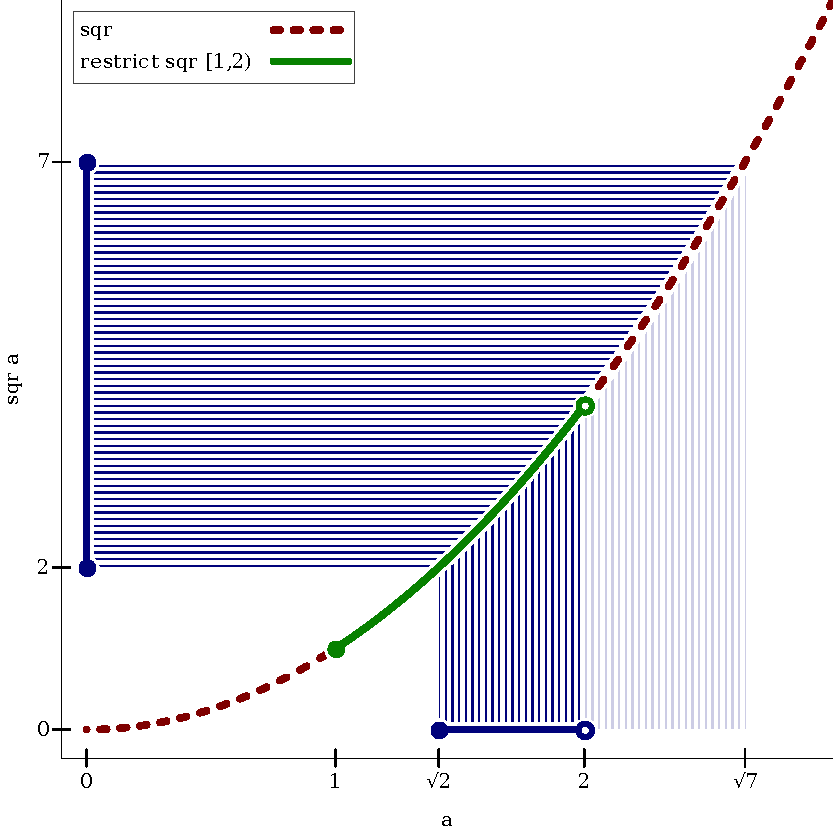
\includegraphics[width=4in]{figures/preimage-by-inverse-image}
\caption[{Computing the preimage of $[2,7]$}]{Computing the preimage of the interval $[2,7]$ under $sqr$ restricted to $[1,2)$, by computing roots and intersecting with $[1,2)$.}
\label{fig:sqr-preimage}
\end{figure}

These facts suggest that we can compute images (or preimages) of intervals under any strictly monotone, surjective $g$ by applying $g$ (or its inverse) to interval endpoints to yield an interval, as in Figure~\ref{fig:sqr-preimage}.
This is evident for endpoints in $A$.
Limit endpoints like $+\infty$ require a larger $\cl{g}$ defined on a compact superset of $A$.

\begin{theorem}[images of intervals by endpoints]
\label{thm:images-of-intervals}
Let $\cl{A}$ and $\cl{B}$ be compact subsets of $\cl{\Re}$, $\cl{g} : \cl{A} \to \cl{B}$ be strictly monotone and surjective, and $g$ be the restriction of $\cl{g}$ to some $A \subseteq \cl{A}$.
For all nonempty $\ivl{a_1,a_2,\alpha_1,\alpha_2} \subseteq A$,
\begin{itemize}
	\item If $\cl{g}$ is increasing, $image~g~\ivl{a_1,a_2,\alpha_1,\alpha_2} = \ivl{\cl{g}~a_1, \cl{g}~a_2,\alpha_1,\alpha_2}$.
	\item If $\cl{g}$ is decreasing, $image~g~\ivl{a_1,a_2,\alpha_1,\alpha_2} = \ivl{\cl{g}~a_2, \cl{g}~a_1,\alpha_2,\alpha_1}$.
\end{itemize}
\end{theorem}
\begin{proof}
Because $\cl{A}$ is compact and totally ordered, every subset of $\cl{A}$ has a lower and an upper bound in $\cl{A}$.
Therefore, the endpoints of every interval subset of $A$ are in $\cl{A}$.

Let $(a_1,a_2] \subseteq A$.
Suppose $\cl{g}$ is strictly increasing; thus $a_1 < a \leq a_2$ if and only if $\cl{g}~a_1 < \cl{g}~a \leq \cl{g}~a_2$, so $image~g~(a_1,a_2] = image~\cl{g}~(a_1,a_2] = (\cl{g}~a_1,\cl{g}~a_2]$.
The remaining cases are similar.
\end{proof}

To use Theorem~\ref{thm:images-of-intervals} to compute preimages under $g$ by computing images under its inverse $g^{-1}$, we must know if $g^{-1}$ is increasing or decreasing.
The following lemma can help.

\begin{lemma}[inverse direction]
\label{lem:inverse-direction}
If $g : A \to B$ is strictly monotone and surjective with inverse $g^{-1} : B \to A$, then $g$ is increasing if and only if $g^{-1}$ is increasing.
\end{lemma}

\begin{example}[nonnegative square]
The extension of $sqr^+ : [0,+\infty) \to [0,+\infty)$, where $sqr^+~a := a \cdot a$, to the compact superdomain $[0,+\infty]$ is
\begin{equation}
\begin{aligned}
	&\cl{sqr^+} : [0,+\infty] \to [0,+\infty] \\
	&	\cl{sqr^+}~a\ := \lim_{a' \to a} sqr^+~a'
		\ =\ if~(a = +\infty)~{+\infty}~(sqr^+~a)
\end{aligned}
\end{equation}
(With respect to $\Re$'s standard topology, which is first-countable, $sqr^+$ is continuous and thus limit-preserving.)
The extension of its inverse $sqrt^+$ is $\cl{sqrt^+} : [0,+\infty] \to [0,+\infty]$, defined similarly, which by Lemma~\ref{lem:inverse-direction} is also strictly increasing.
Thus,
\begin{equation}
\begin{aligned}
	image~sqr^+~[5,+\infty)\ &=\ [\cl{sqr^+}~5,\cl{sqr^+}~{+\infty})
\\
		\ &=\ [25,+\infty)
\\[6pt]
	preimage~(restrict~sqr^+~[1,2))~[2,7]
		\ &=\ [1,2) \i image~sqrt^+~[2,7]
\\
		\ &=\ [1,2) \i [\cl{sqrt^+}~2,\cl{sqrt^+}~7]
\\
		\ &=\ [1,2) \i [\sqrt{2},\sqrt{7}]
\\
		\ &=\ [\sqrt{2},2)
\end{aligned}
\end{equation}
by Theorem~\ref{thm:images-of-intervals} and Lemma~\ref{lem:invertible-function-preimages}.
\exampleqed
\end{example}

%%%%%%%%%%%%%%%%%%%%%%%%%%%%%%%%%%%%%%%%%%%%%%%%%%%%%%%%%%%%%%%%%%%%%%%%%%%%%
%%%%%%%%%%%%%%%%%%%%%%%%%%%%%%%%%%%%%%%%%%%%%%%%%%%%%%%%%%%%%%%%%%%%%%%%%%%%%
%%%%%%%%%%%%%%%%%%%%%%%%%%%%%%%%%%%%%%%%%%%%%%%%%%%%%%%%%%%%%%%%%%%%%%%%%%%%%

\subsection{Two-Argument Primitives}

We do not expect to be able to compute preimages under $\Re \times \Re \pto \Re$ primitives by simply inverting them.
Two-argument invertible real functions are difficult to define and are usually pathological.
Instead, we compute approximate preimages only, using inverses with respect to one argument (with the other held constant).

\begin{definition}[axial inverse]
\label{def:axial-inverse}
Let $g_c : A \times B \to C$.
Functions $g_a : B \times C \to A$ and $g_b : C \times A \to B$ defined so that
\begin{equation}
	g_c~\pair{a,b} = c\ \iff\ g_a~\pair{b,c} = a\ \iff\ g_b~\pair{c,a} = b
\end{equation}
are \mykeyword{axial inverses} with respect to $g_c$'s first and second arguments.
\end{definition}

We call $g_c$ \mykeyword{axis-invertible} or \mykeyword{trijective} when it has axial inverses $g_a$ and $g_b$.
We call $g_a$ the \mykeyword{first axial inverse} of $g_c$ because it is the inverse of $g_c$ along the first axis: $g_a$ with only $c$ varying, or $\fun{c \in C} g_a~\pair{b,c}$, is the inverse of $g_c$ with only $a$ varying, or $\fun{a \in A} g_c~\pair{a,b}$.
Similarly, $g_b$ is the \mykeyword{second axial inverse}.

\begin{example}
\label{ex:plus-axial-inverses}
Let $add_c : \Re \times \Re \to \Re$, $add_c~\pair{a,b} := a+b$.
Its axial inverses are $add_a~\pair{b,c} := c - b$ and $add_b~\pair{c,a} := c - a$.
\exampleqed
\end{example}

We have chosen the axial inverse function types carefully: they are the only types for which $g_c$, $g_a$ and $g_b$ form a cyclic group.

\begin{theorem}[axial inverse cyclic group]
\label{thm:axial-inverse-cyclic-group}
The following statements are equivalent.
\begin{itemize}
	\item $g_c$ has axial inverses $g_a$ and $g_b$.
	\item $g_a$ has axial inverses $g_b$ and $g_c$.
	\item $g_b$ has axial inverses $g_c$ and $g_a$.
\end{itemize}
Equivalently, every axis-invertible function generates a cyclic group of order 3 by inversion in the first axis.
\end{theorem}
\begin{proof}
This is evident from the definition of axial inverse (Definition~\ref{def:axial-inverse}).
\end{proof}

This fact is analogous to how mutual inverses $g$ and $g^{-1}$ form a cyclic group of order 2 generated by inversion.
Similar to using mutual inversion to compute images and preimages under both $sqr^+$ and $sqrt^+$, Theorem~\ref{thm:axial-inverse-cyclic-group} allows computing preimages under two-argument functions related by axial inversion.

\begin{example}
Define $sub_c : \Re \times \Re \to \Re$ by $sub_c~\pair{a,b} := a-b$.
Because $sub_c = add_b$, $sub_a = add_c$ and $sub_b = add_a$.
\exampleqed
\end{example}

Unlike inverses, axial inverses do not provide a direct way to compute exact preimages.
Instead, they provide a way to compute a preimage's smallest rectangular bounding set.

\begin{theorem}[preimage bounds from axial inverse images]
\label{thm:axis-invertible-function-preimages}
Let $A' \subseteq A$, $B' \subseteq B$, $C' \subseteq C$, and $g_c : A \times B \to C$ with axial inverses $g_a$ and $g_b$.
If $g_c' := restrict~g_c~(A' \times B')$, then
\begin{equation}
	preimage~g_c'~C'\ \subseteq\ \lzfcsplit{
		&(A' \i image~g_a~(B' \times C'))\ \times \\
		&(B' \i image~g_b~(C' \times A'))}
\end{equation}
Further, the right-hand side is the smallest rectangular superset.
\end{theorem}
\begin{proof}
The smallest rectangle containing $preimage~g_c'~C'$ is
\begin{equation}
	preimage~g_c'~C'\ \subseteq\ 
		\lzfcsplit{
			&(image~fst~(preimage~g_c'~C'))\ \times \\
			&(image~snd~(preimage~g_c'~C'))}
\end{equation}
Starting with the first set in the product, expand definitions, distribute $fst$, replace $g_c~\pair{a,b} = c$ by $g_a~\pair{b,c} = a$, and simplify:
\begin{displaybreaks}
\begin{align*}
	&image~fst~(preimage~g_c'~C')
\nobreak\\
	&\tab =\ image~fst~\setb{\pair{a,b} \in A' \times B'}{g_c~\pair{a,b} \in C'}
\\
	&\tab =\ \setb{a \in A'}{\Exists{b \in B'} g_c~\pair{a,b} \in C'}
\\
	&\tab =\ \setb{a \in A'}{\Exists{b \in B',c \in C'} g_c~\pair{a,b} = c}
\\
	&\tab =\ \setb{a \in A'}{\Exists{b \in B',c \in C'} g_a~\pair{b,c} = a}
\\
	&\tab =\ \setb{g_a~\pair{b,c}}{b \in B', c \in C', g_a~\pair{b,c} \in A'}
\\
	&\tab =\ A' \i \setb{g_a~\pair{b,c}}{b \in B', c \in C'}
\nobreak\\
	&\tab =\ A' \i image~g_a~(B' \times C')
\end{align*}
\end{displaybreaks}
The second set in the product is similar.
\end{proof}

\begin{figure}[!tb]
\centering
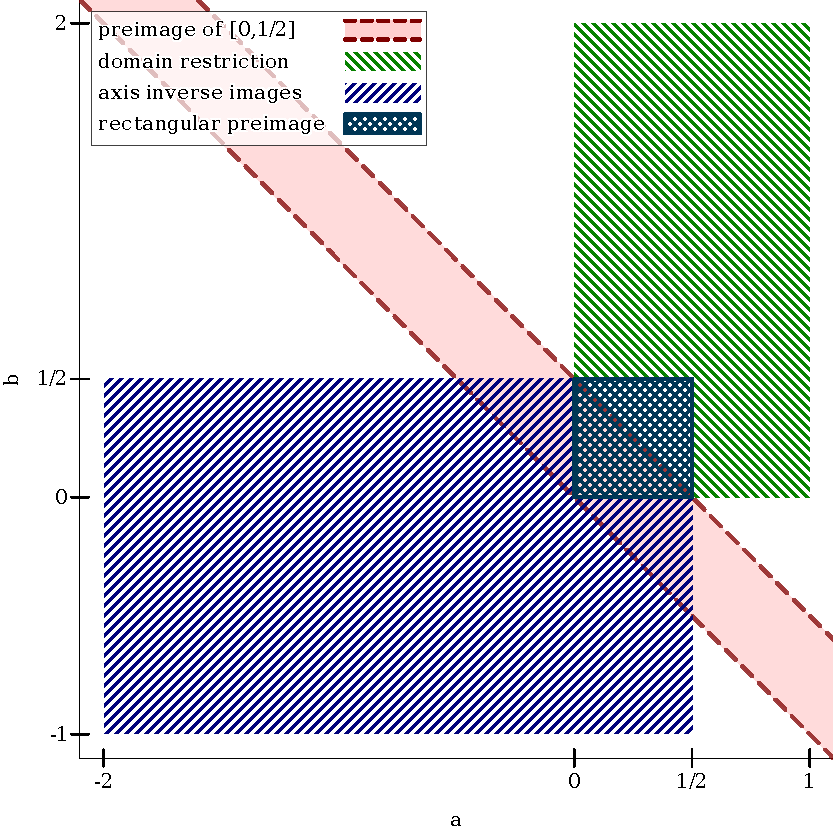
\includegraphics[width=4in]{figures/rect-preimage-by-inverse-images}
\caption[{Computing an approximate preimage of $[0,1{/}2]$}]{Computing an approximate preimage of $[0,\tfrac{1}{2}]$ under addition restricted to $[0,1] \times [0,2]$ (Example~\ref{ex:plus-preimage}).
The preimage is approximated by intersecting the domain with an overapproximation computed using axial inverses.}
\label{fig:plus-preimage}
\end{figure}

\begin{example}
\label{ex:plus-preimage}
Let $add_c' := restrict~add_c~([0,1] \times [0,2])$.
By Theorem~\ref{thm:axis-invertible-function-preimages},
\begin{align*}
	preimage~add_c'~[0,\tfrac{1}{2}]
		&\subseteq \lzfcsplit{
			&([0,1] \i image~add_a~([0,2] \times [0,\tfrac{1}{2}]))\ \times \\
			&([0,2] \i image~add_b~([0,\tfrac{1}{2}] \times [0,1]))}
\\
		&= ([0,1] \i [-2,\tfrac{1}{2}]) \times ([0,2] \i [-1,\tfrac{1}{2}])
\\
		&= [0,\tfrac{1}{2}] \times [0,\tfrac{1}{2}]
\end{align*}
is the smallest rectangular subset of $[0,1] \times [0,2]$ containing the preimage of $[0,\tfrac{1}{2}]$ under $add_c'$.
Figure~\ref{fig:plus-preimage} illustrates the calculation.
\exampleqed
\end{example}

At this point, we have an analogue of Lemma~\ref{lem:invertible-function-preimages}, in that we can compute (approximate) preimages by computing images under (axial) inverses.
Computing images using interval endpoints requires analogues of Lemma~\ref{lem:monotone-implies-invertible} (strictly monotone, surjective implies invertible, continuous), Theorem~\ref{thm:images-of-intervals} (images of intervals by endpoints), and Lemma~\ref{lem:inverse-direction} (inverse direction).

We first need a notion of function properties that hold for one argument for every fixed value of the other argument.
We will say that $g_c : A \times B \to C$ has property $P$ \mykeyword{in its first axis} when $P~(\fun{a \in A} g_c~\pair{a,b})$ for all $b \in B$.
Similarly, $g_c$ has property $P$ \mykeyword{in its second axis} when $P~(\fun{b \in B} g_c~\pair{a,b})$ for all $a \in A$.

Now Lemma~\ref{lem:monotone-implies-invertible}'s analogue is an easy corollary.

\begin{theorem}[strictly monotone, surjective implies axis-invertible, continuous]
\label{thm:uniformly-monotone-implies-invertible}
Let $g_c : A \times B \to C$ for totally ordered $A$, $B$ and $C$.
If $g_c$ is surjective and either strictly increasing or strictly decreasing in each axis, then $g_c$ is axis-invertible; further, it and its axial inverses are continuous.
\end{theorem}
\begin{proof}
XXX: todo
\end{proof}

\begin{example}
In each axis, $add_c$ is surjective and strictly increasing.
In each axis, $sub_c$ is surjective, and is strictly increasing/decreasing in its first/second axis.
Therefore, both are axis-invertible.
\exampleqed
\end{example}

Restriction usually makes a function not surjective in each axis.

\begin{example}
Let $add_c' : [0,1] \times [0,1] \to [0,2]$, defined by restricting $add_c$.
It is surjective, but not in each axis: the range of $\fun{b \in B} add_c'~\pair{0,b}$ is $[0,1]$, not $[0,2]$.
\exampleqed
\end{example}

\begin{figure}[!tb]
\centering
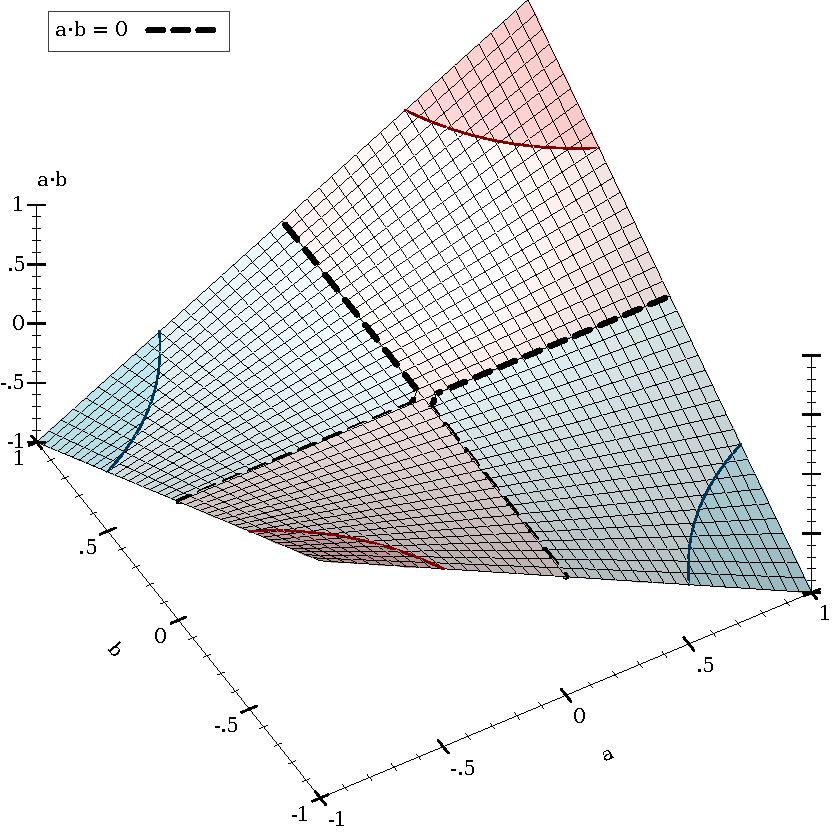
\includegraphics[width=4in]{figures/mul-nonuniform-properties}
\caption[Multiplication on $\Re \times \Re$]{Multiplication on $\Re \times \Re$ is not surjective nor strictly monotone in each axis: $a \cdot 0 = 0$ and $0 \cdot b = 0$ for all $a$ and $b$ (Example~\ref{ex:mul-nonuniform}).
Fortunately, restricted to each open quadrant, multiplication is surjective and strictly increasing or decreasing in each axis.}
\label{fig:mul-nonuniform}
\end{figure}

Fortunately, restriction sometimes does the opposite.

\begin{example}
\label{ex:mul-nonuniform}
Define $mul_c : \Re \times \Re \to \Re$ by $mul_c~\pair{a,b} := a \cdot b$.
It is not surjective nor strictly monotone in each axis because $mul_c~\pair{0,b} = 0$ for all $b \in B$.
(See Figure~\ref{fig:mul-nonuniform}.)
But $mul_c^{++} : (0,+\infty) \times (0,+\infty) \to (0,+\infty)$, and $mul_c$ restricted to the other open quadrants, are surjective and strictly increasing or decreasing in each axis.
\exampleqed
\end{example}

Theorem~\ref{thm:images-of-intervals} justifies computing images of intervals with infinite endpoints under one-argument functions by applying an extended function to the endpoints.
Its two-argument analogue is more involved because extended, two-argument functions may not be defined at every point.

\begin{example}
$add_c$ cannot be extended to $\cl{add_c} : \cl{\Re} \times \cl{\Re} \to \cl{\Re}$ in the same way $sqr^+$ is extended to $\cl{sqr^+}$ because
\begin{equation}
	\lim_{\pair{a',b'} \to \pair{a,b}} add_c~\pair{a',b'}
\end{equation}
diverges when $\pair{a,b}$ is $\pair{-\infty,+\infty}$ or $\pair{+\infty,-\infty}$.
\exampleqed
\end{example}

The previous example suggests that extensions of strictly increasing, two-argument functions are always well-defined except at off-diagonal corners.
This is true, and similar statements hold for axes with other directions, and for more restricted domains.

\begin{theorem}[$\cl{\Re} \times \cl{\Re}$ extension]
\label{thm:two-argument-extensions}
Let $A$, $B$, $C$ be open subsets of $\Re$, and $g_c : A \times B \to C$ be surjective and strictly increasing or decreasing in each axis.
Let $\cl{A}$, $\cl{B}$ and $\cl{C}$ be the closures of $A$, $B$ and $C$ in $\cl{\Re}$.
The following extension is well-defined:
\begin{equation}
\begin{aligned}
	&\cl{g_c} : (\cl{A} \times \cl{B}) \w N \to \cl{C} \\
	&\cl{g_c}~\pair{a,b}\ :=\ \lim_{\pair{a',b'} \to \pair{a,b}} g_c~\pair{a',b'}
\end{aligned}
\end{equation}
where $N := \set{\pair{min~\cl{A},max~\cl{B}},\pair{max~\cl{A},min~\cl{B}}}$ if $g_c$ is increasing in each axis or decreasing in each axis, and
$N := \set{\pair{min~\cl{A},min~\cl{B}},\pair{max~\cl{A},max~\cl{B}}}$ if $g_c$ is increasing/decreasing or decreasing/increasing.
\end{theorem}
\begin{proof}
Suppose $g_c$ is increasing/increasing, and let $xs : \Nat \to A \times B$ be a sequence of $g_c$'s domain values, and $ys := map~g_c~xs$.

Interior case: $xs$ converges to $\pair{a,b} \in A \times B$.
The limit of $ys$ is $g_c~\pair{a,b}$ because $g_c$ preserves limits by its continuity (by Theorem~\ref{thm:uniformly-monotone-implies-invertible}) in the first-countable space $\Re \times \Re$.

Corner case: $xs$ converges to $\pair{max~\cl{A},max~\cl{B}}$.
It thus has a strictly increasing subsequence.
By monotonicity, $ys$ has a strictly increasing subsequence.
Because $ys$ is bounded by $max~\cl{C}$, $\cl{g_c}~\pair{max~\cl{A},max~\cl{B}} = max~\cl{C}$.
A similar argument proves $\cl{g_c}~\pair{min~\cl{A},min~\cl{B}} = min~\cl{C}$.

Border case: $xs$ converges to $\pair{max~\cl{A},b'}$ for some $b' \in B$.
Define
\begin{equation}
	xs'\ :=\ map~(\fun{\pair{a,b}}\pair{g_a~\pair{b',g_c~\pair{a,b}},b'})~xs
\end{equation}
where $g_a$ is $g_c$'s first axial inverse.
Now $ys = map~g_c~xs'$.
Because $xs'$ has a subsequence that is strictly increasing in the first of each pair, and because the second of each pair is the constant $b'$, by monotonicity, $ys$ has a strictly increasing subsequence.
It is bounded by $max~\cl{C}$, so $\cl{g_c}~\pair{max~\cl{A},b'} = max~\cl{C}$.
Similar arguments prove $\cl{g_c}~\pair{min~\cl{A},b'} = min~\cl{C}$, $\cl{g_c}~\pair{a',max~\cl{B}} = max~\cl{C}$, and $\cl{g_c}~\pair{a',min~\cl{B}} = min~\cl{C}$.

The cases for $g_c$'s other possible directions are similar.
\end{proof}

Following the proof of Theorem~\ref{thm:two-argument-extensions}, extensions of two-argument functions can be defined by two corner cases, four border cases, and an interior case.

\begin{example}
Define $pow_c : (0,1) \times (0,+\infty) \to (0,1)$ by $pow_c~\pair{a,b} := exp~(b \cdot log~a)$, which is increasing/decreasing.
Its extension to a subset of $\cl{\Re} \times \cl{\Re}$ is
\begin{equation}
\begin{aligned}
	&\cl{pow_c} : ([0,1] \times [0,+\infty]) \w N \to [0,1] \\
	&\cl{pow_c}~\pair{a,b}\ :=\
		\lzfccase{\pair{a,b}}{
			\pair{0,+\infty} & 0 \\
			\pair{1,0} & 1 \\ 
			\pair{0,b} & 0 \\
			\pair{1,b} & 1 \\
			\pair{a,0} & 1 \\
			\pair{a,+\infty} & 0 \\
			else & pow_c~\pair{a,b}
		}
\end{aligned}
\end{equation}
where $N := \set{\pair{0,0},\pair{1,+\infty}}$.
\exampleqed
\end{example}

The analogue of Theorem~\ref{thm:images-of-intervals} (images of intervals by endpoints) is easiest to state if we have predicates that indicate a function's direction in each axis.
Define $inc_1 : (A \times B \to C) \tto Bool$ so that $inc_1~g$ if and only if $g$ is strictly increasing in its first axis, and similarly $inc_2$ so that $inc_2~g$ if and only if $g$ is strictly increasing in its second axis.

\begin{theorem}[images of rectangles by interval endpoints]
\label{thm:images-of-rectangles}
Let $A,B,C$ be open subsets of $\Re$, and $g_c : A \times B \to C$ be surjective and strictly increasing or decreasing in each axis, with $\cl{g_c}$ as defined in Theorem~\ref{thm:two-argument-extensions}.
If $A' := \ivl{a_1,a_2,\alpha_1,\alpha_2} \subseteq A$ and $B' := \ivl{b_1,b_2,\beta_1,\beta_2} \subseteq B$, then
\begin{equation}
\begin{aligned}
	C'\ :=&\ image~g_c~(\ivl{a_1,a_2,\alpha_1,\alpha_2} \times \ivl{b_1,b_2,\beta_1,\beta_2})
\\
	=&\ \lzfclet{
		\pair{a_1',a_2',\alpha_1',\alpha_2'} & \lzfccond{(inc_1~g_c) & \pair{a_1,a_2,\alpha_1,\alpha_2} \\ else & \pair{a_2,a_1,\alpha_2,\alpha_1}} \\
		\pair{b_1',b_2',\beta_1',\beta_2'} & \lzfccond{(inc_2~g_c) & \pair{b_1,b_2,\beta_1,\beta_2} \\ else & \pair{b_2,b_1,\beta_2,\beta_1}}
	}{\ivl{\cl{g_c}~\pair{a_1',b_1'},\cl{g_c}~\pair{a_2',b_2'},\alpha_1'~and~\beta_1',\alpha_2'~and~\beta_2'}}
\end{aligned}
\end{equation}
\end{theorem}
\begin{proof}
Because $g_c$ is continuous and $A' \times B'$ is a connected set, $C'$ is a connected set, which in $\Re$ is an interval.
Thus, we need to determine only its endpoints and whether it contains each endpoint.

Suppose $g_c$ is increasing/increasing.
In this case, $a_1' = a_1$, $b_1' = b_1$, and so on.
By monotonicity, $C'$ is contained in $[\cl{g_c}~\pair{a_1',b_1'},\cl{g_c}~\pair{a_2',b_2'}]$.
If $\alpha_1'$ or $\beta_1'$ is $false$, $C'$ cannot contain $\cl{g_c}~\pair{a_1',b_1'}$.
If $\alpha_2'$ or $\beta_2'$ is $false$, $C'$ cannot contain $\cl{g_c}~\pair{a_2',b_2'}$.
Therefore $C' = \ivl{\cl{g_c}~\pair{a_1',b_1'},\cl{g_c}~\pair{a_2',b_2'},\alpha_1'~and~\beta_1',\alpha_2'~and~\beta_2'}$.

We still must prove $\pair{a_1',b_1'}$ and $\pair{a_2',b_2'}$ are in $\cl{g_c}$'s domain.
First, recall $\cl{g_c} : (\cl{A} \times \cl{B}) \w N \to \cl{C}$, where $\cl{A}$, $\cl{B}$ and $\cl{C}$ are the closures of $A$, $B$ and $C$, and $N = \set{\pair{min~\cl{A},max~\cl{B}},\pair{max~\cl{A},min~\cl{B}}}$.
Because $A' \subseteq A$ and $B' \subseteq B$, and $A$ and $B$ are open sets, $a_1 \neq max~\cl{A}$, $a_2 \neq \min~\cl{A}$, $b_1 \neq max~\cl{B}$, and $b_2 \neq min~\cl{B}$, so for all $a \in \cl{A}$ and $b \in \cl{B}$,
\begin{equation}
\begin{aligned}
	\pair{a_1,b_1} &\neq \pair{max~\cl{A},b} \hspace{0.5in} & \pair{a_2,b_2} &\neq \pair{min~\cl{A},b} \\
	\pair{a_1,b_1} &\neq \pair{a,max~\cl{B}} \hspace{0.5in} & \pair{a_2,b_2} &\neq \pair{a,min~\cl{B}}
\end{aligned}
\end{equation}
Therefore, $\pair{a_1,b_1} \not\in N$ and $\pair{a_2,b_2} \not\in N$, as desired.

The remaining cases for $g_c$ are similar.
\end{proof}

\begin{example}
Because $inc_1~pow_c$ and $not~(inc_2~pow_c)$,
\begin{align*}
	&image~pow_c~((0,\tfrac{1}{2}] \times [2,+\infty))
\\
	&\ =\ \lzfclet{
		\pair{a_1,a_2,\alpha_1,\alpha_2} & \pair{0,\tfrac{1}{2},false,true} \\
		\pair{b_1,b_2,\beta_1,\beta_2} & \pair{+\infty,2,false,true}
	}{\ivl{\cl{pow_c}~\pair{a_1,b_1},\cl{pow_c}~\pair{a_2,b_2},\alpha_1~and~\beta_1,\alpha_2~and~\beta_2}}
\\
	&\ =\ \ivl{\cl{pow_c}~\pair{0,+\infty},\cl{pow_c}~\pair{\tfrac{1}{2},2},false~and~false,true~and~true}
\\
	&\ =\ \ivl{0,\tfrac{1}{4},false,true}
\\
	&\ =\ (0,\tfrac{1}{4}]
\\[-2.25\baselineskip]
\end{align*}
\exampleqed
\end{example}

To use Theorem~\ref{thm:images-of-rectangles} to compute approximate preimages under some $g_c$ by computing images under its axial inverses, we must know whether each axis of $g_a$ and $g_b$ is increasing or decreasing.
It helps to have an analogue of Lemma~\ref{lem:inverse-direction} (inverse direction).

\begin{theorem}[axial inverse directions]
\label{thm:axial-inverse-direction}
Let $g_c : A \times B \to C$ be surjective and strictly increasing or decreasing in each axis, with axial inverses $g_a$ and $g_b$.
Then
\begin{enumerate}
	\item $inc_1~g_a$ if and only if $(inc_1~g_c)~xor~(inc_2~g_c)$.
	\item $inc_2~g_a$ if and only if $inc_1~g_c$.
\end{enumerate}
\end{theorem}
\begin{proof}
For 1, let $c \in C$, $b_1,b_2 \in B$, $a_1 := g_a~\pair{b_1,c}$ and $a_2 := g_a~\pair{b_2,c}$.
Let $c' := g_c~\pair{a_1,b_2}$; note $c = g_c~\pair{a_1,b_1} = g_c~\pair{a_2,b_2}$.
Suppose $inc_1~g_c$ and $inc_2~g_c$; then $a_1 > a_2 \iff c < c'$ and $b_1 < b_2 \iff c < c'$, so $b_1 < b_2 \iff a_1 > a_2$.
The remaining cases are similar.

For statement 2, fix $b \in B$ and apply Lemma~\ref{lem:inverse-direction}.
\end{proof}

By Theorem~\ref{thm:axial-inverse-direction}, we can use $g_c$'s axis directions to determine $g_a$'s, and by Theorem~\ref{thm:axial-inverse-cyclic-group} (axial inverse cyclic group), use $g_a$'s to determine $g_b$'s.


%%%%%%%%%%%%%%%%%%%%%%%%%%%%%%%%%%%%%%%%%%%%%%%%%%%%%%%%%%%%%%%%%%%%%%%%%%%%%
%%%%%%%%%%%%%%%%%%%%%%%%%%%%%%%%%%%%%%%%%%%%%%%%%%%%%%%%%%%%%%%%%%%%%%%%%%%%%
%%%%%%%%%%%%%%%%%%%%%%%%%%%%%%%%%%%%%%%%%%%%%%%%%%%%%%%%%%%%%%%%%%%%%%%%%%%%%

\subsection{Primitive Implementation}
\label{sec:primitive-implementation}

Because floating-point functions are defined on subsets of $\cl{\Re}$, it would seem we could compute preimages under strictly monotone, real functions by applying their floating-point counterparts to interval endpoints.
This is mostly true, but as with \scheme{real-set-singleton}, we must take care with rounding.
We must also account for floating-point negative zero.

As with all interval arithmetic, to compute sound approximations of interval images, we must round the results \keyword{outward}: round the lower endpoints down, and round the upper endpoints up.
Unlike with most interval arithmetic, soundness is not just a nice theoretical guarantee.
For the lowest-rejection-rate sampling algorithm presented further on, it is critical.

The sampler chooses a random value $a$, restricts $\Omega$ at index $j$ to $[a,a]$ using $\Omega' := unproj~j~\Omega~[a,a]$, and computes a preimage under the program's interpretion as a function, restricted to $\Omega'$.
If in the forward pass, the approximation of the image of $\Omega'$ is not sound, the reverse pass will often falsely compute an empty preimage.

Here is a more concrete example.
As a preimage arrow computation, square root is
\begin{equation}
\begin{aligned}
	&sqrt_{pre} : [0,+\infty) \preto\,[0,+\infty) \\
	&sqrt_{pre}~A\ :=\ \pair{image~sqrt^+~A, preimage~(restrict~sqrt^+~A)}
\end{aligned}
\end{equation}
Suppose $A = [\frac{1}{2},\frac{1}{2}]$, and that the implementation mistakenly computes $image~sqrt^+~[\frac{1}{2},\frac{1}{2}]$ as $[0.7071067811865476,0.7071067811865476]$.
The number $0.7071067811865476$ is the closest 64-bit floating-point number to $\sqrt{\frac{1}{2}}$; i.e. the implementation's floating-point square root is compliant with the IEEE 754 floating-point standard~\cite{cit:ieee-754-2008}.

Suppose that on the reverse phase, we compute the preimage of $\Re$ under $restrict~sqrt^+~[\frac{1}{2},\frac{1}{2}]$.
By Lemma~\ref{lem:invertible-function-preimages}, the implementation of $pre$ should compute
\begin{equation}
\begin{aligned}
	&preimage~(restrict~sqrt^+~[\tfrac{1}{2},\tfrac{1}{2}])~(\Re \i [0.7071067811865476,0.7071067811865476])
\\
	&\tab=\ [\tfrac{1}{2},\tfrac{1}{2}] \i image~sqr^+~[0.7071067811865476,0.7071067811865476]
\end{aligned}
\end{equation}
If it again uses compliant floating-point arithmetic but does not round outward, it computes
\begin{equation}
	[\tfrac{1}{2},\tfrac{1}{2}] \i [0.5000000000000001,0.5000000000000001]\ =\ \emptyset
\end{equation}
In fact, an implementation that does not round intervals outward would falsely compute $\emptyset$ for about half of the floating-point numbers between $0.0$ and $1.0$.

The IEEE 754 floating-point standard mandates a settable rounding mode, and that common operations must use it to determine which of the nearest floating-point numbers to round to.
Unfortunately, there is no portable way to set the rounding mode.
In Racket, we have a few other options.
\begin{enumerate}
	\item Use \scheme{math/bigfloat}, which wraps the MPFR arbitrary-precision floating-point library~\cite{cit:fousse-2007-mpfr}, which \emph{does} provide a way to set the rounding mode for its operations.
	\item Use the \scheme{math/flonum} library's functions for \keyword{double-doubles}, which are two nonoverlapping floating-point numbers that when added together represent a number with a 105-bit significand~\cite{cit:shewchuk-1997}.
	Convert flonums to double-doubles, operate on them, and manually round the high-order number of the result up or down based on the sign of the low-order number.
	\item Use the \scheme{math/flonum} library's \scheme{flnext} and \scheme{flprev} to bump the endpoints up or down.
\end{enumerate}
We use option 2 for functions with 105-bit implementations, such as arithmetic, $exp$ and $log$, and otherwise use option 3.

For option 3, how far the endpoints are bumped up or down depends on the maximum error in the output of the function's floating-point implementation.
For example, we use the normal distribution's inverse cumulative density function $F_N^{-1}$ and (its inverse $F_N$) to transform uniformly distributed random numbers (i.e. each $\omega~j$) into normally distributed random numbers.
As a preimage arrow computation, it is
\begin{equation}
\begin{aligned}
	&normal!inv!cdf_{pre} : (0,1)~\preto~\Re \\
	&normal!inv!cdf_{pre}~A\ :=\ \pair{image~F_N^{-1}~A, preimage~(restrict~F_N^{-1}~A)}
\end{aligned}
\label{eqn:normal-inv-cdf-pre}
\end{equation}
Racket's \scheme{math/distributions} library implements $F_N^{-1}$ with \scheme{flnormal-inv-cdf} and $F_N$ with \scheme{flnormal-cdf}, whose outputs are always within four floating-point numbers of the exact outputs.
The implementation of $normal_{pre}$ therefore bumps lower endpoints down by $4$ and upper endpoints up by $4$.

For the code in this section, we use a \scheme{/rndu} suffix (read ``with rounding up'') for the names of functions that round up, and a \scheme{/rndd} for the name of functions that round down.
In Racket, prefixing floating-point functions with \scheme{fl} is conventional, so the name of the floating-point addition function that rounds down is \scheme{fl+/rndd}, and the name of the floating-point square root function that rounds up is \scheme{flsqrt/rndu}.

\begin{figure*}[tb!]\centering
\begin{schemedisplay}
;; Represents an R -> R bijection, its direction, domain and range
(struct: Bijection
    ([inc? : Boolean] [domain : Real-Set] [range : Real-Set]
     [gb/rndd : (Flonum -> Flonum)] [gb/rndu : (Flonum -> Flonum)]
     [ga/rndd : (Flonum -> Flonum)] [ga/rndu : (Flonum -> Flonum)]))
<blank-line>
(: bijection-inverse (Bijection -> Bijection))
;; Returns the inverse of a bijection (see Lemma 8.5)
(define (bijection-inverse g)
  (match-define (Bijection inc? X Y gb/rndd gb/rndu ga/rndd ga/rndu) g)
  (Bijection inc? Y X ga/rndd ga/rndu gb/rndd gb/rndu))
<blank-line>
(: real-image (Boolean (Flonum -> Flonum) (Flonum -> Flonum) Real-Set
                -> Real-Set))
;; Returns a sound approximation of the image of A under g (Theorem 8.4)
(define (real-image inc? g/rndd g/rndu A)
  (match-define (Real-Set a1 a2 a1? a2?) A)
  (cond [inc?  (Real-Set (g/rndd a1) (g/rndu a2) a1? a2?)]
        [else  (Real-Set (g/rndd a2) (g/rndu a1) a2? a1?)]))
<blank-line>
(: bijection-image (Bijection Real-Set -> (U Empty-Set Real-Set)))
;; Computes the image of A under bijection g
(define (bijection-image g A)
  (match-define (Bijection inc? X Y gb/rndd gb/rndu _ _) g)
  (let ([A  (real-set-intersect A X)])
    (if (empty-set? A)
        empty-set
        (real-set-intersect Y (real-image inc? gb/rndd gb/rndu A)))))
<blank-line>
(: bijection-preimage (bijection Real-Set Real-Set -> (U Empty-Set Real-Set)))
;; Returns an approximate preimage of B under g restricted to A (Lemma 8.3)
(define (bijection-preimage g A B)
  (match-define (Bijection inc? X Y _ _ ga/rndd ga/rndu) g)
  (let ([A  (real-set-intersect A X)]
        [B  (real-set-intersect B Y)])
    (if (or (empty-set? A) (empty-set? B))
        empty-set
        (real-set-intersect A (real-image inc? ga/rndd ga/rndu B)))))
\end{schemedisplay}
\bottomhrule
\caption[Computing images and preimages under real functions]{Typed Racket code for computing images and preimages under strictly monotone, surjective real functions.}
\label{fig:bijection-implementation}
\end{figure*}

Figure~\ref{fig:bijection-implementation} lists code that computes sound image and preimage approximations under strictly monotone, surjective real functions.
Such functions are represented by instances of \scheme{Bijection}.
Each instance contains a \scheme{Boolean} indicating whether the function is increasing, its domain, range, an implementation with rounding down and up, and an inverse implementation with rounding down and up.
For example,
\begin{center}\singlespacing
\begin{schemedisplay}
(define pos-sqr-bij
  (Bijection #t nonnegative-reals nonnegative-reals
             flsqr/rndd flsqr/rndu
             flsqrt/rndd flsqrt/rndu))
<blank-line>
(define sqrt-bij
  (bijection-inverse pos-sqr-bij))
\end{schemedisplay}
\end{center}
The preimage arrow computation \scheme{sqrt-pre} computes \scheme{(bijection-image sqrt-bij A)} in the forward phase and \scheme{(bijection-preimage sqrt-bij A B)} in the reverse phase.

A simple example shows how floating-point's signed zeros can cause problems: the implementation of the reciprocal function.
Let $\cl{recip^+}$ be the extension of $recip^+ : (0,+\infty) \to (0,+\infty)$ to the compact superdomain $[0,+\infty]$, defined by
\begin{equation}
\begin{aligned}
	&\cl{recip^+} : [0,+\infty] \to [0,+\infty] \\
	&\cl{recip^+}~a\ :=\ \lim_{a' \to a}~recip^+~a'\ =\ 
		\lzfccase{a}
		{
			0 & +\infty \\
			+\infty & 0 \\
			else & recip^+~a \\
		}
\end{aligned}
\end{equation}
Suppose we implement it this way:
\begin{center}\singlespacing
\begin{schemedisplay}
(define pos-recip-bij
  (Bijection #f positive-reals positive-reals
             (λ (a) (fl//rndd 1.0 a)) (λ (a) (fl//rndu 1.0 a))
             (λ (a) (fl//rndd 1.0 a)) (λ (a) (fl//rndu 1.0 a))))
\end{schemedisplay}
\end{center}
Because $recip^+$ is surjective, $image~recip^+~(0,+\infty) = (0,+\infty)$.
With this implementation, we get the expected result only when the left endpoint is \emph{positive} floating-point zero, or \scheme{+0.0}:
\begin{center}\singlespacing
\begin{schemedisplay}
> (bijection-image pos-recip-bij (Real-Set +0.0 +inf.0 #f #f))
(Real-Set 0.0 +inf.0 #f #f)
<blank-line>
> (bijection-image pos-recip-bij (Real-Set -0.0 +inf.0 #f #f))
empty-set
\end{schemedisplay}
\end{center}
The issue is that \scheme{(fl/ 1.0 +0.0)} returns \scheme{+inf.0}, but \scheme{(fl/ 1.0 -0.0)} returns \scheme{-inf.0}, as per the IEEE 754 floating-point standard.
The implementation should compute
\begin{equation}
	image~recip^+~(0,+\infty)\ =\ (\cl{recip^+}~{+\infty}, \cl{recip^+}~0)\ =\ (0,+\infty)
\end{equation}
but tries to return $(0,-\infty)$, which is the empty set.

In interval arithmetic, the typical solution is to allow \scheme{+0.0} only as a lower endpoint, and \scheme{-0.0} as only as an upper endpoint~\cite{cit:hickey-2001-interval}.
We have not determined whether this solution generalizes to nonarithmetic functions, however, so we define
\begin{center}\singlespacing
\begin{schemedisplay}
(define (pos-recip/rndd a)
  (if (fl= a 0.0) +inf.0 (fl/ 1.0 a)))
\end{schemedisplay}
\end{center}
and similarly \scheme{pos-recip/rndu}, and define \scheme{pos-recip-bij} in terms of these functions.

\begin{figure*}[p!]\centering
\begin{schemedisplay}
;; Represents an R x R -> R trijection, its directions, domain and range
(struct: Trijection
 ([inc1? : Boolean] [inc2? : Boolean]
  [domain1 : Real-Set] [domain2 : Real-Set] [range : Real-Set]
  [gc/rndd : (Flonum Flonum -> Flonum)] [gc/rndu : (Flonum Flonum -> Flonum)]
  [ga/rndd : (Flonum Flonum -> Flonum)] [ga/rndu : (Flonum Flonum -> Flonum)]
  [gb/rndd : (Flonum Flonum -> Flonum)] [gb/rndu : (Flonum Flonum -> Flonum)]))
<blank-line>
(: real2d-image (Boolean Boolean
                 (Flonum Flonum -> Flonum)
                 (Flonum Flonum -> Flonum)
                 Real-Set Real-Set -> Real-Set))
;; Returns a sound approximation of the image of AxB under g (Theorem 8.20)
(define (real2d-image inc1? inc2? g/rndd g/rndu A B)
  (define-values (a1 a2 a1? a2?)
    (match-let ([(Real-Set a1 a2 a1? a2?)  A])
      (cond [inc1?  (values a1 a2 a1? a2?)]
            [else   (values a2 a1 a2? a1?)])))
  (define-values (b1 b2 b1? b2?)
    (match-let ([(Real-Set b1 b2 b1? b2?)  B])
      (cond [inc2?  (values b1 b2 b1? b2?)]
            [else   (values b2 b1 b2? b1?)])))
  (Real-Set (g/rndd a1 b1) (g/rndu a2 b2) (and a1? b1?) (and a2? b2?)))
<blank-line>
(: trijection-preimage (Trijection Real-Set Real-Set Real-Set
                         -> (Values (U Empty-Set Real-Set)
                                    (U Empty-Set Real-Set))))
;; Returns an approximate preimage of C under g restricted to AxB
;; (Theorem 8.11, Theorem 8.22)
(define (trijection-preimage g A B C)
  (match-define (Trijection gc-inc1? gc-inc2? X Y Z
                            _ _ ga/rndd ga/rndu gb/rndd gb/rndu) g)
  (define ga-inc1? (xor gc-inc1? gc-inc2?))
  (define ga-inc2? gc-inc1?)
  (define gb-inc1? (xor ga-inc1? ga-inc2?))
  (define gb-inc2? ga-inc1?)
  (let ([A  (real-set-intersect A X)]
        [B  (real-set-intersect B Y)]
        [C  (real-set-intersect C Z)])
    (if (or (empty-set? A) (empty-set? B) (empty-set? C))
        (values empty-set empty-set)
        (values (real-set-intersect
                 A (real2d-image ga-inc1? ga-inc2? ga/rndd ga/rndu B C))
                (real-set-intersect
                 B (real2d-image gb-inc1? gb-inc2? gb/rndd gb/rndu C A))))))
\end{schemedisplay}
\bottomhrule
\caption[Computing images and preimages under two-dimensional real functions]{Typed Racket code for computing images and preimages under two-dimensional real functions that are surjective and strictly increasing or decreasing in each axis.}
\label{fig:trijection-implementation}
\end{figure*}

Figure~\ref{fig:trijection-implementation} lists code that computes sound image and preimage approximations under two-dimensional real functions that are surjective and strictly increasing or decreasing in each axis.
Such functions are represented by instances of \scheme{Trijection}.
Each instance contains two \scheme{Boolean} values indicating whether each axis is increasing, its axis domains, its range, an implementation with rounding down and up, and two axial inverse implementations with rounding down and up.
For example, the implementations of addition and subtraction are
\begin{center}\singlespacing
\begin{schemedisplay}
(define add-trij
  (Trijection #t #t reals reals reals
              fl+/rndd fl+/rndu
              flrev-/rndd flrev-/rndu
              fl-/rndd fl-/rndu))
<blank-line>
(define sub-trij
  (trijection-second-inverse add-trij))
\end{schemedisplay}
\end{center}
where \scheme{flrev-/rndd} implements $add_a~\pair{b,c} := c - b$ with rounding down.

\subsection{Piecewise Monotone Primitives}
\label{sec:piecewise-monotone-primitives}

Using $\ifpre$, it is easy to provide primitives that are piecewise monotone with finitely many pieces.
We first need predicates to distinguish the parts, so we define
\begin{equation}
\begin{aligned}
	&negative?\pre : \Re \preto Bool \\
	&negative?\pre\ :=\ predicate\pre~(-\infty,0]~(0,+\infty)
\end{aligned}
\label{eqn:negative-pre}
\end{equation}
as well as $positive?\pre$ in the same way.

From $sqr^+\pre$ (nonnegative square) and $neg\pre$ (negation) primitives, we define
\begin{equation}
\begin{aligned}
	sqr\pre&\ :=\ \ifpre~negative?\pre~(neg\pre~\comppre~sqr^+_{pre})~sqr^+\pre
\\
	sqr\ppre&\ :=\ \eta\ppre~sqr\pre
\end{aligned}
\end{equation}
We then extend $\meaningofconv{\cdot}\ppre$ by the rule $\meaningofconv{sqr~\mathit{e}}\ppre\ :=\ \meaningofconv{\mathit{e}}\ppre~\compppre~sqr\ppre$.
Equivalently, we could provide $sqr^+$, $neg$ and $negative?$ as primitives and define
\begin{equation}
	sqr~a\ :=\ strict!if~(negative?~a)~(sqr^+~(neg~a))~(sqr^+~a)
\end{equation}
as a standard library function for probabilistic programs.

From implementations of multiplication restricted to each open quadrant, or $mul^{++}\pre$, $mul^{+-}\pre$, $mul^{-+}\pre$ and $mul^{--}\pre$, we can define multiplication on all of $\Re \times \Re$ with
\begin{equation}
\begin{aligned}
	mul\pre &\ := \
		\lzfcsplit{\ifpre~
			&(fst\pre~\comppre~positive?\pre) \\
			&(\lzfcsplit{\ifpre~
				&(snd\pre~\comppre~positive?\pre) \\
				&mul^{++}\pre \\
				&(\lzfcsplit{\ifpre~
					\lzfcsplit{&(snd\pre~\comppre~negative?\pre) \\
						&mul^{+-}\pre \\
						&(const\pre~0)))}
				}
			} \\
			&...\ \text{[similar code using $mul^{-+}\pre$ and $mul^{--}\pre$]}\ ...
		}
\\
	mul\ppre &\ :=\ \eta\ppre~mul\pre
\end{aligned}
\end{equation}
and extend $\meaningofconv{\cdot}\ppre$ by the rule $\meaningofconv{\mathit{e_1} \cdot \mathit{e_2}}\ppre\ :=\ \meaningofconv{\pair{\mathit{e_1},\mathit{e_2}}}\ppre~\compppre~mul\ppre$.


\section{Sampling Methods}

Chapter~\ref{ch:preimage1} defines the preimage refinement algorithm (Definition~\ref{def:preimage-refinement}), which repeatedly splits a partition of the program domain, restricts the program to each part, and refines each part by computing a preimage.
While it appears to converge for programs that terminate with probability $1$, it is inefficient.
Good accuracy requires fine discretization, which is exponential in the number of discretized axes.
For example, a nonrecursive program that contains only 10 uses of $random$ would need to partition 10 axes of $\Omega$.
Splitting each axis into only 4 disjoint intervals yields a partition of $\Omega$ of size $4^{10} = 1,048,576$.

Fortunately, Bayesian practitioners tend to be satisified with sampling methods, which are usually more efficient than enumeration methods.
To approximately answer conditional queries, it suffices to sample within the preimage of the condition set.
More precisely, if $g := \meaningofconv{\mathit{p}}\pmap$, we can answer almost any query $\Pspec{B' | B}$ by sampling within $A := preimage~g~B$, if the probability of $A$ is positive.

\begin{figure*}[tb!]\centering
\subfloat[Exact preimage of $B$]{%
\label{fig:preimage-refinement:exact}%
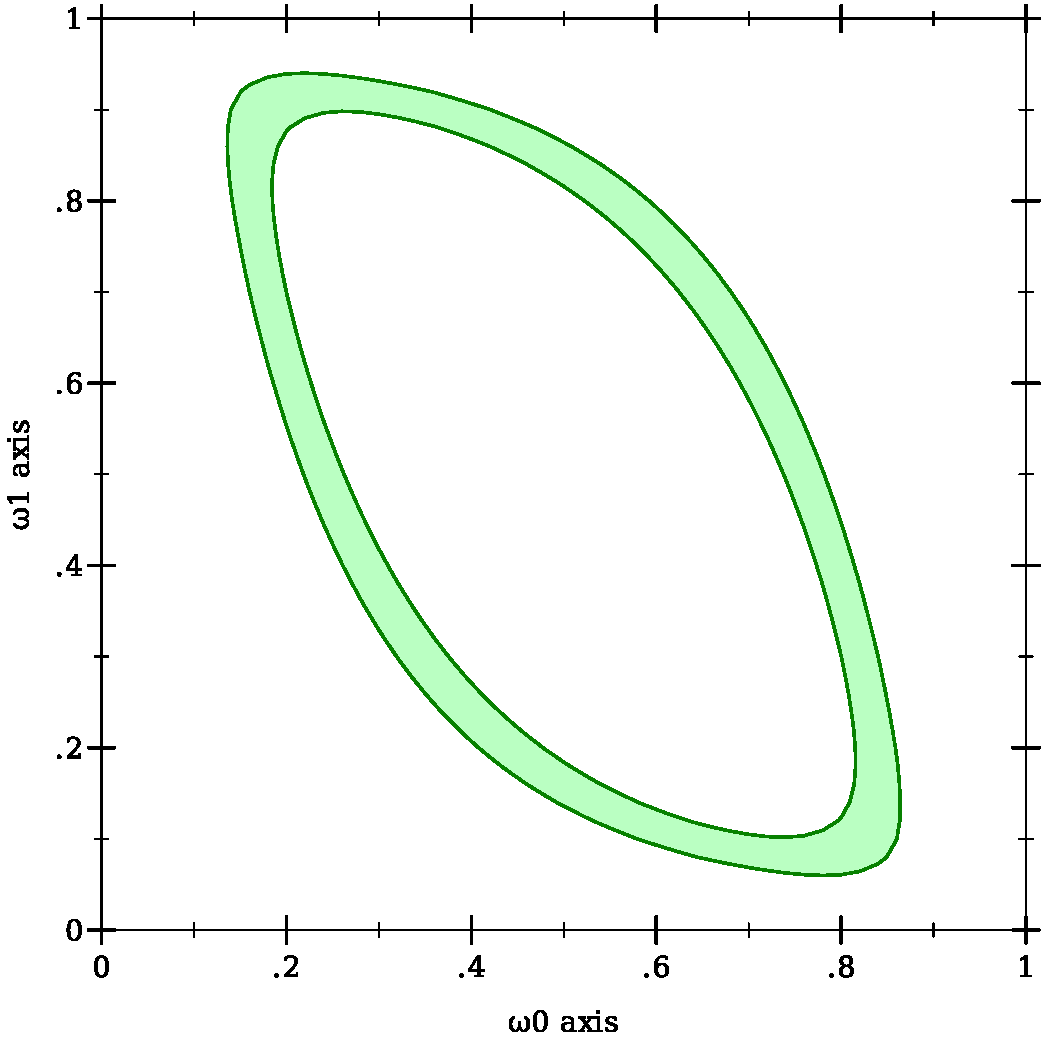
\includegraphics[width=\subfigurewidth]{figures/refinement/constrained-norm-norm-source-00}%
}%
\betweenrefinementfigurehspace%
\subfloat[Parts sampled from a rectangular cover instead of enumerated]{%
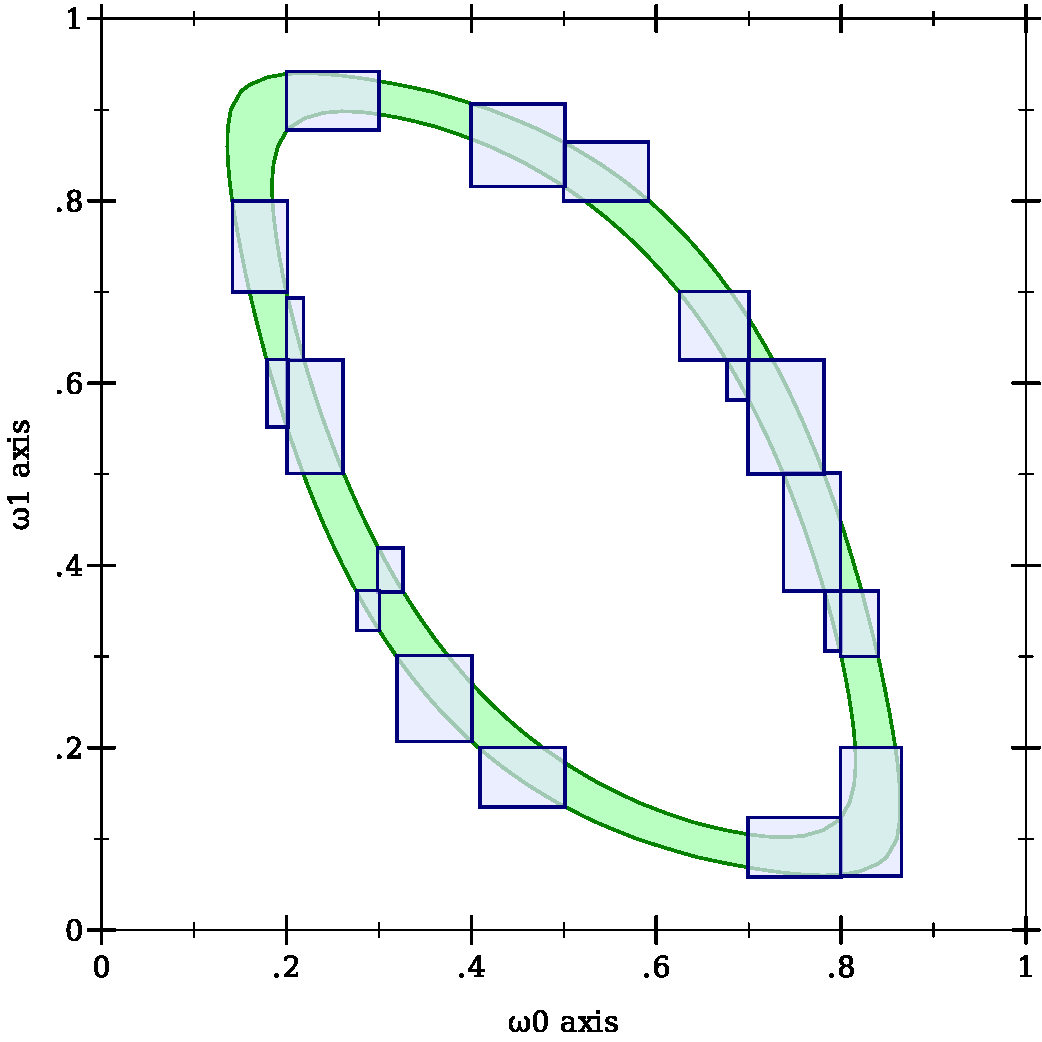
\includegraphics[width=\subfigurewidth]{figures/refinement/constrained-norm-norm-source-sample}%
}%
\betweenrefinementfigurehspace%
\subfloat[Points sampled within the parts]{%
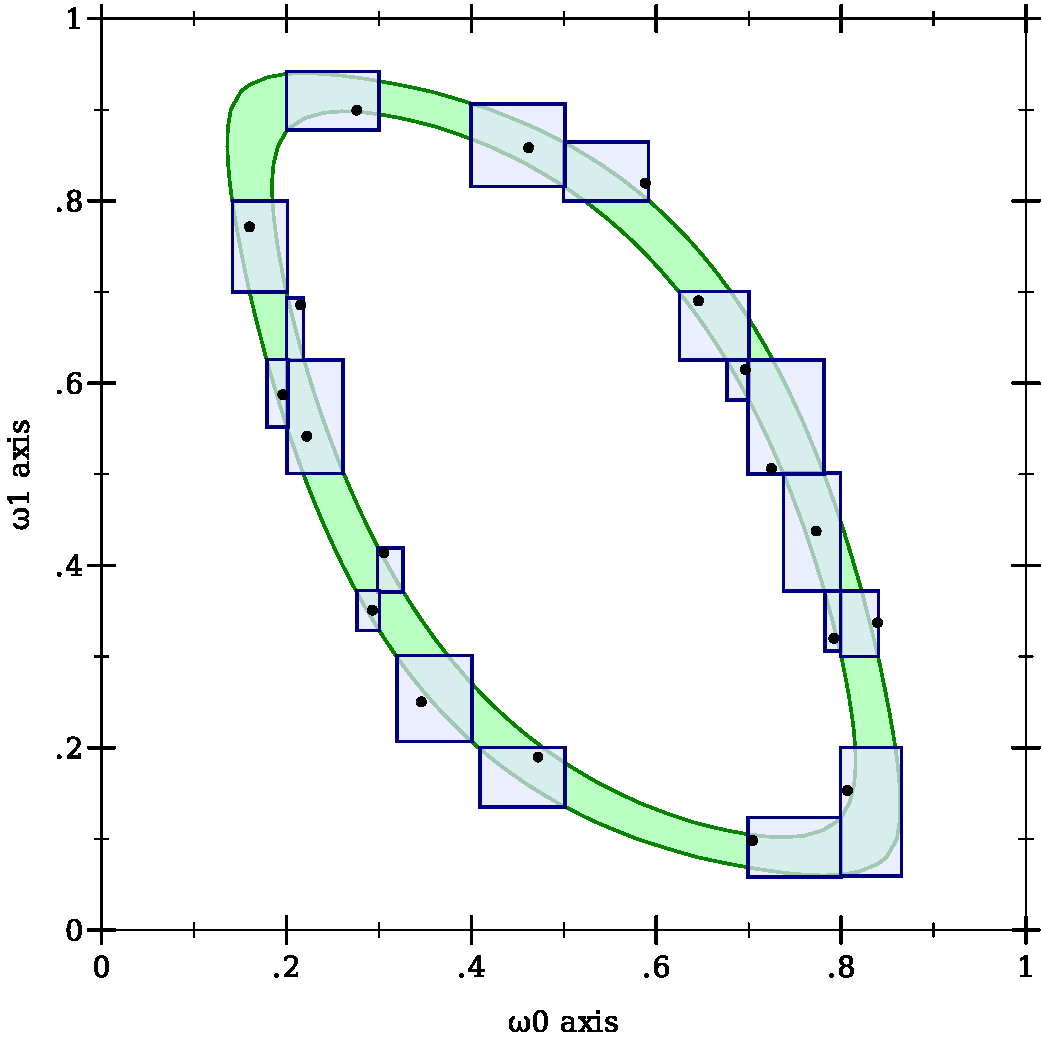
\includegraphics[width=\subfigurewidth]{figures/refinement/constrained-norm-norm-source-sample-point}%
}

\caption[Preimage refinement sampling]{A more efficient alternative to the preimage refinement algorithm.
Instead of enumerating a rectangular cover, its parts are sampled, and each part is then sampled from.
Points that lie outside the exact preimage (which is easy to test) are rejected.
}
\label{fig:preimage-refinement-sampling}
\end{figure*}

It is easy to sample within $A$ by sampling within $\Omega$ and rejecting samples not in $A$.
To determine whether samples are in $A$, we can use the interpretation of the program $\mathit{p}$ as a bottom* arrow computation $f := \meaningofconv{\mathit{p}}_\pbot$.
Unfortunately, the time required to accept a fixed number of samples also tends to be exponential in the number of dimensions.
To solve this problem, we sample within a rectangular cover of $A$, as computed by preimage refinement, instead of within $\Omega$.
But we do not need to enumerate the cover's parts, as Figure~\ref{fig:preimage-refinement-sampling} illustrates: for each sample, we first sample a part, and then sample a value within the part.

\subsection{Partitioned Sampling}

More generally, without considering probabilistic programming at all, we want to sample values in a probability space $X,P$ by first sampling a part from a partition of $X$ and then sampling from that part.\footnote{This is not \emph{stratified} sampling, which samples a fixed number of times from each partition.}

First, to restrict probability measures to measurable, positive-probability sets and renormalize them, we define
\begin{equation}
\begin{aligned}
	&condition : Set~X \pto [0,1] \tto Set~X \tto Set~X \pto [0,1] \\
	&condition~P~A\ :=\ \fun{A' \in domain~P} P~(A' \i A)~{/}~P~A
\end{aligned}
\end{equation}

\begin{definition}[partitioned sampling]
\label{def:partitioned-sampling}
Let $X,P$ be an arbitrary probability space, $N$ be an at-most-countable index set, and $s : N \to Set~X$ be a partition of $X$ into $|N|$ measurable parts. The following procedure samples from $X$:
\begin{enumerate}
	\item Choose $n \in N$ with probability $P~(s~n)$.
	\item Choose $a \in s~n$ according to $condition~P~(s~n)$.
\end{enumerate}
\end{definition}

It is not hard to show that partitioned sampling chooses an $a \in X$ according to $P$.

\begin{example}[partitioned sampling from a standard normal]
\label{ex:partitioned-sampling}
Let $P$ be the standard normal distribution's probability measure.
To sample according to $P$, let $N := \set{neg,pos}$ and $s = [neg \mapsto (-\infty,0], pos \mapsto (0,+\infty)]$, and define $Q : N \to Set~\Re \pto [0,1]$ by
\begin{equation}
\begin{aligned}
	Q~neg~A\ &=\ P~((-\infty,0] \i A)~{/}~\tfrac{1}{2} \\
	Q~pos~A\ &=\ P~((0,+\infty) \i A)~{/}~\tfrac{1}{2}
\end{aligned}
\end{equation}
Then
\begin{enumerate}
	\item Choose $n = neg$ or $n = pos$, each with probability $\frac{1}{2}$.
	\item Choose $a \in s~n$ according to $Q~n$.\exampleqed
\end{enumerate}
\end{example}

Partitioned sampling has two weaknesses.
First, it requires $P~(s~n)$ to be easy to compute for all $n \in N$.
If this were true, we would not need to sample in the first place---i.e. it assumes a solution to the overall problem we are trying to solve.
Second, it assumes sampling according to $condition~P~(s~n)$ is easy, which is also not reasonable, as sampling according to a conditioned distribution is a subproblem we are trying to solve.

But suppose we could easily sample a partition index according to a different distribution over $N$, and according to a different distribution over part $s~n$ for each $n \in N$. Doing so and returning weighted samples to adjust for the differences in distribution comprises \mykeyword{partitioned importance sampling}.

First, to restrict a probability measure $P$ to a measurable set $A$ \emph{without} renormalizing it, we define
\begin{equation}
\begin{aligned}
	&subcond : Set~X \pto [0,1] \tto Set~X \tto Set~X \pto [0,1] \\
	&subcond~P~A\ :=\ \fun{A' \in domain~P} P~(A' \i A)
\end{aligned}
\end{equation}
This returns a \keyword{subprobability measure}: a measure whose largest output is less than $1$.

\begin{definition}[partitioned importance sampling]
\label{def:partitioned-importance-sampling}
Suppose we have
\begin{itemize}
	\item An arbitrary probability space $X,P$.
	\item An at-most-countable index set $N$.
	\item A probability mass function $p : N \to [0,1]$ such that $p~n > 0$ for all $n \in N$.
	\item A partition $s : N \to Set~X$ of $X$ into $|N|$ measurable parts.
	\item Candidate probability measures $Q : N \to Set~X \pto [0,1]$, one for each partition.
\end{itemize}
To sample from $X$ according to $P$,
\begin{enumerate}
	\item Choose $n \in N$ with probability $p~n$.
	\item Choose $a \in X$ according to $Q~n$.
	\item Compute $w := \dfrac{1}{p~n} \cdot diff^+~(subcond~P~(s~n))~(Q~n)~a$.
	\item Return the weighted sample $\pair{a,w}$.
\end{enumerate}
\end{definition}

The function $diff^+~(subcond~P~(s~n))~(Q~n)$, with type $X \to [0,+\infty)$, is a \keyword{Radon-Nikod\'ym\footnote{Pronounced ``RADon neekohDIM,'' and named after Austrian mathematician Johann Radon and Polish mathematician Otto Nikod\'ym.} derivative}.
If $P$ has density $f$, $Q~n$ has density $g$, and $a \in s~n$ implies $g~a > 0$, then\footnote{The equality in~\eqref{eqn:diff-is-actually-easy} holds $(Q~n)$-almost everywhere.}
\begin{equation}
	diff^+~(subcond~P~(s~n))~(Q~n)~a\ =\ if~(a \in s~n)~(f~a~{/}~g~a)~0
\label{eqn:diff-is-actually-easy}
\end{equation}
Appendix~\ref{ch:sampling-algorithm-proofs} has formal definitions and more details.
We use $diff^+$ in a more general sense, but in this section, it is usually fine to think of its return values as quotients of densities.

An importance sampling algorithm is correct when all expected values computed using its weighted samples are the equal to the true expected values.
This is true of partitioned importance sampling under reasonable conditions, which are analogous to the support of $subcond~P~(s~n)$ being no larger than that of $Q~n$.
The formal statement of the theorm and its proof are in Appendix~\ref{ch:sampling-algorithm-proofs}.

Partitioned importance sampling allows quite a lot of freedom: parts can be chosen with arbitrary nonzero probability, and each part can have its own candidate distribution, which may be defined on a superset of the part.

\begin{figure}[!tb]
\centering
\subfloat[Unweighted samples]{
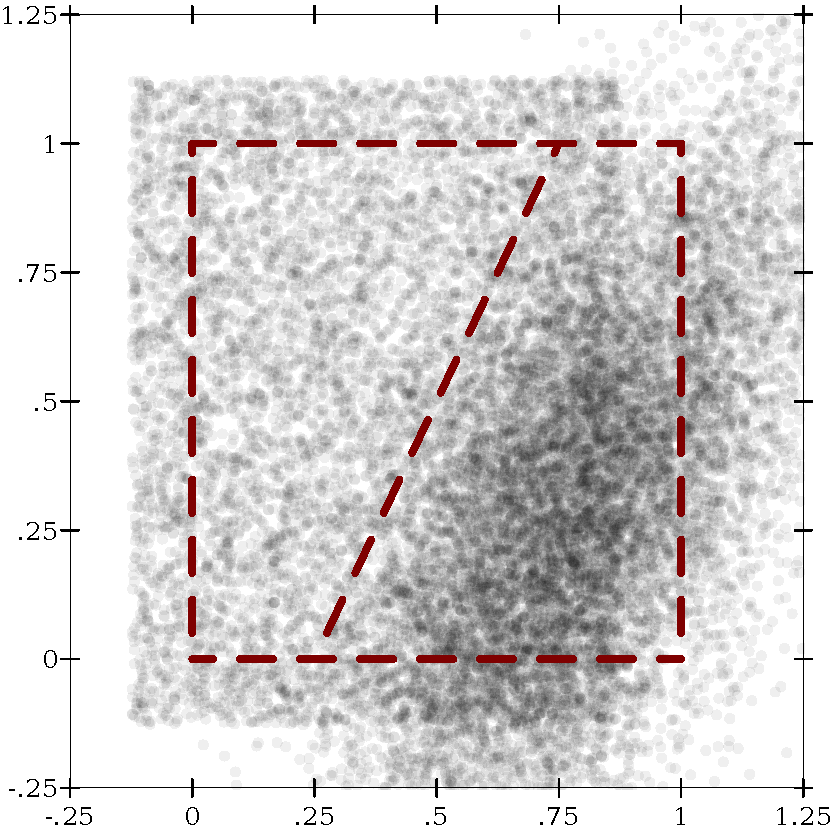
\includegraphics[width=3in]{figures/pimp-sampling-unweighted}
}
\hspace{0.1in}
\subfloat[Resampled by weight]{
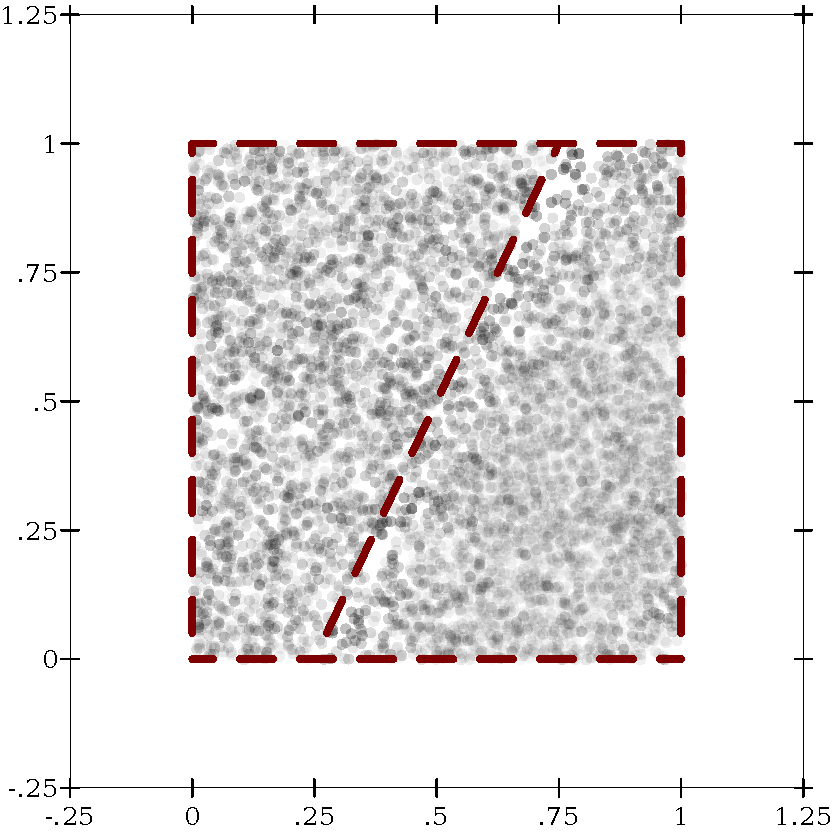
\includegraphics[width=3in]{figures/pimp-sampling-weighted}
}
\caption[Sampling uniformly in a partioned unit square]{Partitioned importance sampling used to sample uniformly in a partition of the unit square, using two overlapping candidate distributions.}
\label{fig:pimp-sampling-2d}
\end{figure}

\begin{example}[2D partitioned importance sampling]
\figref{fig:pimp-sampling-2d} shows the result of partitioned importance sampling in a partition of the unit square.
In this instance,
\begin{itemize}
	\item $X := [0,1] \times [0,1]$ and $P$ is the uniform measure on $X$ (i.e. area).
	\item $N := \set{left,right}$.
	\item $p := [left \mapsto 0.4, right \mapsto 0.6]$.
	\item $s~left = \setb{\pair{x,y} \in X}{y > 2 \cdot x - \frac{1}{2}}$, similarly for $s~right$.
	\item $Q~left$ is the uniform measure on a superset of $s~left$, and $Q~right$ is a multivariate Gaussian measure centered at $\pair{0.8,0.3}$.
\end{itemize}
The implementation does not actually construct most of these objects. It constructs
\begin{itemize}
	\item A density function $f : \Re \times \Re \tto [0,+\infty)$ to represent $P$.
	\item A family of predicates $s? : N \tto X \tto Bool$ to decide $a \in s~n$.
	\item Candidate densities $g : N \tto X \tto [0,+\infty)$ to represent $Q$.
\end{itemize}
It computes weights using $diff^+~(subcond~P~(s~n))~(Q~n)~a\ =\ f~a~{/}~g~n~a$ when $s?~n~a = true$.
It directly represents only $N$ and $p$, but we will find even this to be infeasible shortly.
\exampleqed
\end{example}

Two properties make the preceeding example simple.
First, the partition has finitely many parts.
Second, the measures $subcond~P~(s~n)$ and $Q~n$ have densities, which ensures $diff^+~(subcond~P~(s~n))~(Q~n)$ exists and is easy to compute.

When sampling in the domain of programs, neither property holds in general.

\subsection{Partitioning Probabilistic Program Domains}

For the random source part $\Omega := J \to [0,1]$ of probabilistic language domains, which consists of infinite binary trees of reals, it is not clear that partitioned importance sampling is applicable.
The main problem is that it is difficult to prove that any given infinite-dimensional Radon-Nikod\'ym derivative exists.

Fortunately, we can prove they exist if the two measures differ in only finitely many axes.
More precisely, let $P_1 : Set~\Omega \to [0,1]$ and $P_2 : Set~\Omega \to [0,1]$ be probability measures, and $J' \subseteq J$ be a finite set of tree indexes.
Suppose $P_1$ can be factored into a distribution $P_1'$ over finite prefixes $J' \to [0,1]$ and a distribution over suffixes $(J \w J') \to [0,1]$, and $P_2'$ can be similarly factored into $P_2'$ and \emph{the same} distribution over suffixes.
Then, under reasonable conditions (which are analogous to the support of $P_1'$ being no larger than that of  $P_2'$), $diff^+~P_1~P_2$ exists and can be computed using $diff^+~P_1'~P_2'$.
Appendix~\ref{ch:sampling-algorithm-proofs} contains a formal statement and proof.

To ensure $subcond~P~(s~n)$ and $Q~n$ differ in only finitely many axes, we partition $\Omega$ according to branch traces.
Because only finitely branches may be taken, each branch trace corresponds with a program that reads any $\omega \in \Omega$ at only finitely many indexes $J' \subseteq J$.

In the remainder of this subsection, assume a fixed program $\mathit{p}$. Let $f := \meaningofconv{\mathit{p}}_\pbot : \pair{\pair{\Omega,T},\pair{}} \pbotto Y$ be its interpretation as a bottom* arrow computation, with maximal domain $A^*$.
Define $T^* := image~(fst~\arrowcomp~snd)~A^*$ as its \mykeyword{maximal branch trace set} and
$\Omega^* := image~(fst~\arrowcomp~fst)~A^*$ as its \mykeyword{maximal random source set}.

We need a notion of the random sources that agree with a given branch trace $t \in T$; i.e. those $\omega \in \Omega$ for which $f~\pair{\pair{\omega,t},\pair{}} \neq \bot$.

\begin{definition}[induced random sources]
\label{def:induced-random-sources}
Let $t \in T$ be a branch trace. The \mykeyword{random sources induced by $t$} are a subset of $\Omega$ defined by
$\Omega' := \setb{\omega \in \Omega}{f~\pair{\pair{\omega,t},\pair{}} \neq \bot}$.
\end{definition}

Equivalently, $\Omega'$ is the set of $\omega \in \Omega$ for which $\pair{\pair{\omega,t},\pair{}} \in A^*$.

[XXX: graph of induced partition from program $if~(random < random)~true~false$?]

\begin{theorem}
\label{thm:t-max-induce-nonempty}
Let $t \in T$ induce $\Omega'$. $\Omega' \neq \emptyset$ if and only if $t \in T^*$.
\end{theorem}
\begin{proof}
By definition of $T^*$, $\Omega' \neq \emptyset$ if and only if there is an $\omega \in \Omega'$ such that $\pair{\pair{\omega,t},\pair{}} \in  A^*$.
\end{proof}

Using $T$ as the partition index set and defining the partition's parts as induced random sources almost works, in the sense that the required Radon-Nikod\'ym derivatives exist.
Unfortunately, we cannot use $T$ or $T^*$ as the partition index set because many branch traces can induce the same random sources.

\begin{example}
For the program
\begin{equation}
	if~(random < p)~0~random
\end{equation}
there are at least two branch traces in the program's maximal domain: $t_0 := [j_0 \mapsto true, * \mapsto \bot]$ and $t_1 := [j_0 \mapsto false, * \mapsto \bot]$.
There is also $[j_0 \mapsto false, left~j_0 \mapsto true, * \mapsto \bot]$, because it agrees with every execution that $[j_0 \mapsto false, * \mapsto \bot]$ agrees with.
In fact, there are infinitely many branch traces in $T^*$ that induce the same random sources as either $t_0$ or $t_1$.
[XXX: tree diagrams?]
\exampleqed
\end{example}

We need to find a subset of branch traces whose induced random sources are disjoint.
The main idea is to define equivalence classes of branch traces that induce the same random sources, and use the ``smallest'' branch trace in each class as a part index.

To identify the ``smallest'' trace in each class, we must define an ordering over them.
One fairly natural way is to say a branch trace is smaller than another when it describes fewer branch decisions; i.e. its tree has fewer non-$\bot$ elements.
Two branch traces that differ by returning respectively $true$ and $false$ for the same $j$ may represent different execution paths, so they must be incomparable.

\begin{definition}[brach trace partial order]
$t_1 \leq t_2$ when for all $j \in J$, $t_1~j = \bot$ or $t_1~j = t_2~j$.
\end{definition}

To find the minimum of a set of equivalent traces, it helps to be able to compute the greatest lower bound, or infimum.
We claim that this function does so:
\begin{equation}
\begin{aligned}
	&trace!inf : Set~T \tto T \\
	&trace!inf~T'\ :=\ \fun{j \in J}
		\lzfccase{proj~j~T'}{
			\set{b} & b \\
			else & \bot
		}
\end{aligned}
\end{equation}

\begin{theorem}[trace infimum]
Let $T' \subseteq T$ and $t_* := trace!inf~T'$.
Then
\begin{itemize}
	\item For all $t' \in T'$, $t_* \leq t'$.
	\item For all $t \in T$, if for all $t' \in T'$, $t \leq t'$, then $t \leq t_*$.
\end{itemize}
\end{theorem}
\begin{proof}
Let $t' \in T'$ and $j \in J$.
If $proj~j~T' = \set{b}$ for $b \in Bool_\bot$, then $t_*~j = t'~j = b$.
Otherwise, $t_*~j = \bot$.
Thus $t_* \leq t'$.

Let $t \in T$ and suppose that for all $t' \in T'$, $t \leq t'$.
Let $j \in J$.
If $proj~j~T' = \set{b}$, then there are two cases: $t~j = \bot$, or $t~j = t_*~j = b$.
Otherwise there exists a $t' \in T'$ such that $t~j \neq t'~j$, so $t~j = \bot$.
Thus $t \leq t_*$.
\end{proof}

Any two comparable traces in $T^*$ induce the same random sources.

\begin{theorem}[comparable implies equivalent]
\label{thm:comparable-implies-same-sources}
Let $t_1,t_2 \in T^*$ induce $\Omega_1$, $\Omega_2$.
If $t_1 \leq t_2$ or $t_2 \leq t_1$, then $\Omega_1 = \Omega_2$.
\end{theorem}
\begin{proof}
It suffices to consider $t_1 \leq t_2$; the $t_2 \leq t_1$ case follows from reflexivity of $(=)$.

Suppose $\omega \in \Omega_1$, so $f~\pair{\pair{\omega,t_1},\pair{}} \neq \bot$.
Let $J' \subseteq J$ such that $j \in J'$ if and only if $\pair{\omega,t_1}$ agrees with the $\convifpbot$ subcomputation at index $j$.
For all $j \in J'$, $t_1~j \neq \bot$, so $t_2~j = t_1~j$ by definition of $(\leq)$.
Therefore, $\pair{\omega,t_2}$ also agrees with every $\convifpbot$ subcomputation at every index $j \in J'$, so $f~\pair{\pair{\omega,t_2},\pair{}} \neq \bot$.
Therefore $\omega \in \Omega_2$, so $\Omega_1 \subseteq \Omega_2$.

Suppose $\omega \notin \Omega_1$.
Let $J' \subseteq J$ such that $j \in J'$ if and only if $t_1~j \neq \bot$.
Because $f~\pair{\pair{\omega,t_1},\pair{}} = \bot$, there exists a $j \in J'$ such that the $\convifpbot$ subcomputation at index $j$ disagrees with $\pair{\omega,t_1}$.
Because $t_1~j = t_2~j$ by definition of $(\leq)$, the $\convifpbot$ subcomputation at index $j$ also disagrees with $\pair{\omega,t_2}$, so $f~\pair{\pair{\omega,t_2},\pair{}} = \bot$.
Therefore $\omega \notin \Omega_2$, so $\Omega_2 \subseteq \Omega_1$.
\end{proof}

\begin{corollary}[infimum in $T^*$ implies equivalent]
Let $t_1,t_2 \in T^*$ induce $\Omega_1$,$\Omega_2$, and define $t_* := trace!inf~\set{t_1,t_2}$.
If $t_* \in T^*$, then $\Omega_1 = \Omega_2$.
\end{corollary}

If $T^*$ is partitioned into equivalence classes of traces that induce the same random sources, each part in the partition contains a smallest member with respect to $(\leq)$.

\begin{theorem}
Let $t \in T^*$ induce $\Omega'$, $T'$ be the largest subset of $T^*$ that induces $\Omega'$, and $t_* := trace!inf~T'$.
Then $t_* \in T'$.
\end{theorem}
\begin{proof}
Let $\omega \in \Omega'$.
By definition of $trace!inf$, every $\convifpbot$ subcomputation agrees with $\pair{\omega,t_*}$.
Therefore $f~\pair{\pair{\omega,t_*},\pair{}} \neq \bot$, so $t_*$ induces $\Omega'$.
\end{proof}

\begin{theorem}[infimum not in $T^*$ implies disjoint]
\label{thm:infimum-not-in-T*}
Let $t_1,t_2 \in T^*$ induce $\Omega_1$,$\Omega_2$, and define $t_* := trace!inf~\set{t_1,t_2}$.
If $t_* \notin T^*$, then $\Omega_1 \i \Omega_2 = \emptyset$.
\end{theorem}
\begin{proof}
Let $T_1$,$T_2$ be the largest subsets of $T^*$ that induce $\Omega_1$, $\Omega_2$.
Let $t_{1*} := trace!inf~T_1$ and $t_{2*} := trace!inf~T_2$.
Because $t_* \notin T^*$, $t_{1*} \neq t_{2*}$.

Let $\omega \in \Omega_1$.
For every $j \in J$ for which $t_{1*}~j \neq \bot$, there is an $\convifpbot$ subcomputation at index $j$ that agrees with $\pair{\omega,t_{1*}}$.
But because $t_{2*} \neq t_{1*}$, there exists a $j \in J$ for which an $\convifpbot$ subcomputation at index $j$ disagrees with $\pair{\omega,t_{2*}}$.
Therefore $\omega \notin \Omega_2$.
By a symmetric argument, $\omega \in \Omega_2$ implies $\omega \notin \Omega_1$.
\end{proof}

We can get our sought-after index set by defining the set of smallest branch traces.

\begin{definition}[minimal branch traces]
The set of \mykeyword{minimal branch traces} $T_*$ is the set of minimal elements in $T^*$, or
\begin{equation}
	T_*\ :=\ \setb{t_1 \in T^*}{\Forall{t_2 \in T^*} t_2 \leq t_1 \implies t_2 = t_1}
\end{equation}
\end{definition}

\begin{theorem}
$T_*$ induces $\Omega^*$.
\end{theorem}
\begin{proof}
Let $t \in T^*$ induce $\Omega'$ and $T'$ be the largest subset of $T^*$ that induces $\Omega'$.
Its minimum $t_* := trace!inf~T'$ is in $T_*$.
\end{proof}

\begin{theorem}[$T_*$ partitions]
\label{thm:minimal-induces-partition}
Let $t_1,t_2 \in T_*$ induce respectively $\Omega_1$ and $\Omega_2$.
If $t_1 \neq t_2$, then $\Omega_1 \i \Omega_2 = \emptyset$.
\end{theorem}
\begin{proof}
Let $t_* := trace!inf~\set{t_1,t_2}$.
Because $t_1$ and $t_2$ are minimal, $t_* \notin T^*$.
By Theorem~\ref{thm:infimum-not-in-T*}, $\Omega_1 \i \Omega_2 = \emptyset$.
\end{proof}

We can thus sample a partition index $t \in T_*$, which induces a unique part from a partition of $\Omega^*$.

A program's minimal branch trace set $T_*$ contains only the actual branches taken when running the program on every $\omega \in \Omega^*$.
Therefore, one way to sample from $T_*$ with the correct probability---at least, for programs that halt with probability $1$---would be to choose an $\omega \in \Omega$ uniformly, and run the program on $\omega$ while recording each branch decision.

But this sampling scheme has problems similar to those of partitioned sampling (Definition~\ref{def:partitioned-sampling}).
First, it assumes the probabilities of branch traces, which are the probabilities of the $\Omega^*$ subsets they induce, are easy to compute.
Second, we are interested in sampling from an \emph{arbitrarily low-probability subset} of $\Omega^*$, which may be covered by the partition induced by an \emph{arbitrarily low-probability subset} of $T_*$.

It appears we have a chicken-and-egg problem, in that
\begin{enumerate}
	\item Sampling in a small subset of $\Omega^*$ requires sampling in a small subset of $T_*$.
	\item Sampling in a small subset of $T_*$ requires sampling in a small subset of $\Omega^*$.
\end{enumerate}
Fortunately, if we allow ourselves subsets of a larger set than $T_*$, and allow ourselves to sample within overapproximating covers of $\Omega^*$ subsets, we can use approximate preimage computation to sample from $T_*$ and $\Omega^*$ subsets simultaneously.

\subsection{Approximate Partitions of Probabilistic Program Domains}

The idea is to define a set of branch traces $T_+$ that is derived only from a program's shape, not its actual executions.
We ensure that $T_* \subseteq T_+$, and that every $t \in T_+ \w T_*$ induces $\emptyset$, so that $T_+$ induces the same partition as $T_*$.
We define an algorithm for sampling from $T_+$, which does not require running a probabilistic program on any $\omega \in \Omega$.
We then extend this algorithm to use preimage computation to sample in arbitrarily good approximations of small subsets of $T_*$ and $\Omega^*$.

\begin{figure*}[!tb]\centering
\smallmathfont
\subfloat[Branch index arrow. Computations return a lazy tree of type $Idxs$, of feasible branch decisions, ignoring the actual values of $if$ conditions. The arrow is directly implementable in any $\lambda$-calculus.]{
\begin{minipage}{0.98\textwidth}
\begin{align*}
\begin{aligned}[t]
	&\begin{aligned}[t]
		Idxs \ ::= &\ \pair{} \gor \pair{Idxs,Idxs} \\
					&\gor if!idxs~J~(1 \tto Idxs)~(1 \tto Idxs) \\
	\end{aligned} \\
\\[-6pt]
	&\begin{aligned}[t]
		&\arrowarr\pbi : (x \tto y) \tto (J \tto Idxs) \\
		&\arrowarr\pbi~f~j\ :=\ \pair{}
	\end{aligned} \\
\\[-6pt]
	&\begin{aligned}[t]
		&(\arrowcomp\pbi) : (J \tto Idxs) \tto (J \tto Idxs) \tto (J \tto Idxs) \\
		&(i_1~\arrowcomp\pbi~i_2)~j \ :=\ \pair{i_1~(left~j), i_2~(right~j)}
	\end{aligned} \\
\\[-6pt]
	&\begin{aligned}[t]
		&(\arrowpair\pbi) : (J \tto Idxs) \tto (J \tto Idxs) \tto (J \tto Idxs) \\
		&(i_1~\arrowcomp\pbi~i_2)~j \ :=\ \pair{i_1~(left~j), i_2~(right~j)}
	\end{aligned} \\
\end{aligned}
&\tab\ \ 
\begin{aligned}[t]
	&\begin{aligned}[t]
		&\arrowif\pbi : (J \tto Idxs) \tto (J \tto Idxs) \tto (J \tto Idxs) \tto (J \tto Idxs) \\
		&\arrowif\pbi~i_1~i_2~i_3~j \ := \ 
			\lzfclet{
				idxs_2 & \fun{0} i_2~(left~(right~j)) \\
				idxs_3 & \fun{0} i_3~(right~(right~j))
			}{\pair{i_1~j, if!idxs~j~idxs_2~idxs_3}}
	\end{aligned} \\
\\[-6pt]
	&\begin{aligned}[t]
		&\arrowlazy\pbi : (1 \tto (J \tto Idxs)) \tto (J \tto Idxs) \\
		&\arrowlazy\pbi~i~j \ := \ i~0~j
	\end{aligned} \\
\\[-6pt]
	&\begin{aligned}[t]
		&random\pbi : J \tto Idxs \\
		&random\pbi~j \ := \ \pair{}
	\end{aligned} \\
\end{aligned}
\end{align*}
\vspace{3pt}
\hrule
\end{minipage}
\label{fig:collecting-semantics:arrow}
}

\subfloat[The stochastic function $sample!traces$ samples a $T'$, and returns $T'$ and its probability.]{
\begin{minipage}{0.98\textwidth}
\begin{equation*}
\begin{aligned}
	&sample!traces : Idxs \to \pair{\Re,Rect~T}
\\
	&sample!traces~idxs\ :=\ sample!traces^*~idxs~\pair{1,T}
\\[6pt]
	&sample!traces^* : Idxs \tto \pair{\Re,Rect~T} \tto \pair{\Re,Rect~T}
\\
	&\lzfcsplit[@{}l@{}l@{}]{
		&sample!traces^*~\pair{}~pt &\ :=\ pt
\\
		&sample!traces^*~\pair{idxs_1,idxs_2}~pt &\ :=\ 
			\lzfclet{
				pt' & sample!traces^*~idxs_1~pt
			}{sample!traces^*~idxs_2~pt'}
\\
		&sample!traces^*~(if!idxs~j~idxs_2~idxs_3)~\pair{p_t,T'} &\ :=\ 
			\lzfclet{
				\pair{p_b,b} & sample!branch~Bool_\bot \\
				pt' & \pair{p_t \cdot p_b, unproj~j~T'~\set{b}}
			}{\lzfccase{b}{
				true & sample!traces^*~(idxs_2~0)~pt' \\
				false & sample!traces^*~(idxs_3~0)~pt' \\
				\bot & pt'
				}
			}
	}
\end{aligned}
\end{equation*}
\vspace{3pt}
\hrule
\end{minipage}
\label{fig:collecting-semantics:sample-traces}
}

\caption[Branch index collecting semantics]{Branch index collecting semantics.}
\label{fig:collecting-semantics}
\end{figure*}

Defining $T_+$ in terms of a program's branching shape requires an additional abstract interpretation.
\figref{fig:collecting-semantics:arrow} defines the \mykeyword{indexes arrow}.
Its type is $J \tto Idxs$, which does not refer to a domain or codomain type of program values because its computations do not receive or compute program values.
Instead, they build lazy trees of possible branching decisions, ignoring the actual values of $if$ conditions.
For example, lifted, pure functions are interpreted as $\fun{j} \pair{}$, which takes the function's computation index and returns no decisions.
Composition and pairing of subcomputations $i_1$ and $i_2$ both return $\pair{i_1~(left~j),i_2~(right~j)}$: a node with two children that contain the feasible branch decisions in their subcomputations.

Only $ifte\pbi$ does more than simple structural recursion: it returns $if!idxs~j~idxs_2~idxs_3$ to represent a decision at computation index $j$.
The children $idxs_2$ and $idxs_3$ are lazy, abstract representations of the $if$'s branches.
Like a concrete execution, a branch trace sampler is expected to compute and recur through only one of them.

Figure~\ref{fig:collecting-semantics:sample-traces} defines $sample!traces$, which, to make its extension for use with preimage refinement easier, samples \emph{rectangles} of branch traces given an $idxs : Idxs$.
It returns a pair $\pair{p_t,T'}$, where $T'$ is the sampled rectangle and $p_t$ is the probability with which it was chosen.
It assumes a stochastic procedure $sample!branch : Set~Bool_\bot \tto \pair{\Re,Bool_\bot}$, where $sample!branch~B$ returns any member of $B$ with some nonzero, constant probability.
At index $j$, for the branch choice $\pair{p_b,b} := sample!branch~Bool_\bot$, $T'$ is restricted using $unproj~j~T'~\set{b}$.

Although $sample!traces$ returns rectangles, it is easy to transform one into a single trace using $trace!inf$; i.e. $trace!inf~(snd~(sample!traces~idxs))$ samples a branch trace.

Let $idxs := \meaningofconv{\mathit{p}}\pbi~j_0$.

\begin{definition}[feasible branch traces]
The \mykeyword{feasible branch traces} $T_+$ are those $t \in T$ for which $\Pspec{t = trace!inf~(snd~(sample!traces~idxs))} > 0$.
\end{definition}

Because $sample!traces^*$ imposes a total order on evaluation, any terminating application of it induces a total order on the indexes $j$ in applications matching $if!idxs~j~idxs_2~idxs_3$.
Let $j_1, j_2, ..., j_n$ be those indexes, with corresponding branch choices $b_1,b_2,...,b_n$.
Define $T'_1,T'_2,...,T'_n$ by $T'_0 := T$ and $T'_i := unproj~j_i~T'_{i-1}~\set{b_i}$.

\begin{theorem}[$sample!traces$ soundness]
$T_* \subseteq T_+$.
\end{theorem}
\begin{proof}
Let $t \in T_*$.
It suffices to show that there exists an $n$ and a sequence of branch choices $b_1,b_2,...,b_n$ for which $t = trace!inf~T'_n$.

First, we prove by induction the seemingly weaker statement that there exist $n$ and branch choices for which $t \in T'_n$.
Let $j_1,j_2,...,j_n$ be the in-order indexes at which $t~j_i \neq \bot$.
Clearly $t \in T'_0 = T$.
If $t \in T'_{i-1}$, then $b_i := t~j_i$ implies $t \in T'_i = unproj~j_i~T'_{i-1}~\set{b_i}$.

For any $j \in \set{j_1,j_2,...,j_n}$, $\set{t~j} = proj~j~T'_n$.
For any other $j$, $t~j = \bot$ and $proj~j~T'_n = Bool_\bot$.
By definition of $trace!inf$, therefore $t = trace!inf~T'_n$.
\end{proof}

For $T_+$ to induce a partition, every $t \in T_+ \w T_*$ must induce $\emptyset$.

\begin{theorem}[$sample!traces$ non-$\emptyset$-unique]
For all $t \in T_+$, if $t \notin T_*$ then $t$ induces $\emptyset$.
\end{theorem}
\begin{proof}
Let $j_1,j_2,...,j_n$ and $b_1,b_2,...,b_n$ for a terminating evaluation of $sample!traces^*~idxs~\pair{1,T}$.

Suppose $T'_n \i T_* = \emptyset$.
Then there exists an $i$ such that $T'_{i-1} \i T_* \neq \emptyset$ and $T'_i \i T_* = \emptyset$.
Thus $b_i \notin proj~j_i~T_*$, so $f$ does not agree with any $t \in T'_i$.

Let $t := trace!inf~T'_n$, which by definition of $trace!inf$ and $sample!traces^*$ is in $T'_n$.
Because $T'_n \subseteq T'_i$, $f$ does not agree with $t$, so $t$ induces $\emptyset$.
\end{proof}

\begin{corollary}[$sample!traces$ partitioning]
$T_+$ induces a partition of $\Omega^*$.
\end{corollary}


To be used in partitioned importance sampling, the probability returned by $sample!traces$ must be correct.

\begin{theorem}[$sample!traces$ correctness]
If $\pair{p_t',T'} := sample!traces~idxs$, then $\Pspec{T'} = p_t'$.
\end{theorem}
\begin{proof}
Let $p_{b_1},p_{b_2},...,p_{b_n}$ be the probabilities returned from $sample!branch$ for $b_1,b_2,...,b_n$.
The probability of $b_1,b_2,...,b_n$ is thus $p_t' := p_{b_1} \cdot p_{b_2} \cdot ... \cdot p_{b_n}$.
Because the transformation from $b_1,b_2,...,b_n$ to $T'_n$ is injective, $\Pspec{T'_n} = p_t'$.
\end{proof}

Further, $sample!traces$ should terminate with probability $1$.

\begin{theorem}[$sample!traces$ termination]
$sample!traces~idxs$ terminates with probability $1$.
\end{theorem}
\begin{proof}
For each branch choice $b_i$, there is a nonzero probability that $b_i = \bot$, which is a recursion base case.
\end{proof}


We finally have a way to use partitioned importance sampling to sample within the preimage of some set $B$.
Define
\begin{equation}
	f\ :=\ \meaningofconv{\mathit{p}}_\pbot~j_0
\hspace{0.5in}
	h'\ :=\ {\meaningofconv{\mathit{p}}}'\ppre~j_0
\hspace{0.5in}
	idxs\ :=\ \meaningofconv{\mathit{p}}\pbi~j_0
\end{equation}
to interpret $\mathit{p}$ as a bottom arrow computation, an approximating preimage arrow computation, and a lazy tree of feasible branch decisions.
Define $refine~A := ap\ppre'~(h'~A)~B$.
Then
\begin{enumerate}
	\item Let $\pair{p_t,T'} := sample!traces~idxs$.
	\item Let $t := trace!inf~T'$.
	\item Let $A' := refine~((\Omega \times \set{t}) \times \set{\pair{}})$.
	\item Let $\Omega' := image~(fst~\arrowcomp~fst)~A'$. If $\Omega' = \emptyset$, reject.
	\item Choose $\omega \in \Omega'$ according to $Q~t$. If $f~\pair{\pair{\omega,t},\pair{}} \notin B$, reject.
	\item Compute weight $w := \dfrac{1}{p_t} \cdot diff^+~(subcond~P~\Omega'')~(Q~t)~\omega$, where $\Omega''$ is the set of random sources induced by $t$.
\end{enumerate}
Computing $diff^+~(subcond~P~\Omega'')~(Q~t)$ does not require $\Omega''$, as we will demonstrate shortly.

Samples are rejected for two reasons.
The first is when $\Omega' = \emptyset$ because $sample!trace$ overapproximates.
The second is when $\omega \in \Omega'$ but $\omega \notin \Omega''$ because $h'$ overapproximates.
To reduce the rejection rate, we must reduce overapproximation as much as possible.
We can address both causes by partitioning $\Omega$ more finely than the partition induced by branch traces.
Doing so requires an update to the indexes arrow and another sampling algorithm.

\begin{figure*}[!tb]\centering
\smallmathfont
\begin{align*}
\begin{aligned}[t]
	&\begin{aligned}[t]
		Idxs \ ::= &\ \pair{} \gor \pair{Idxs,Idxs} \\
					&\gor if!idxs~J~(1 \tto Idxs)~(1 \tto Idxs) \\
					&\gor random!idxs~J \\
	\end{aligned} \\
\\[-6pt]
	&\begin{aligned}[t]
		&\arrowarr\pbi : (x \tto y) \tto (J \tto Idxs) \\
		&\arrowarr\pbi~f~j\ :=\ \pair{}
	\end{aligned} \\
\\[-6pt]
	&\begin{aligned}[t]
		&(\arrowcomp\pbi) : (J \tto Idxs) \tto (J \tto Idxs) \tto (J \tto Idxs) \\
		&(i_1~\arrowcomp\pbi~i_2)~j \ :=\ \pair{i_1~(left~j), i_2~(right~j)}
	\end{aligned} \\
\\[-6pt]
	&\begin{aligned}[t]
		&(\arrowpair\pbi) : (J \tto Idxs) \tto (J \tto Idxs) \tto (J \tto Idxs) \\
		&(i_1~\arrowcomp\pbi~i_2)~j \ :=\ \pair{i_1~(left~j), i_2~(right~j)}
	\end{aligned} \\
\end{aligned}
&\tab\ \ 
\begin{aligned}[t]
	&\begin{aligned}[t]
		&\arrowif\pbi : (J \tto Idxs) \tto (J \tto Idxs) \tto (J \tto Idxs) \tto (J \tto Idxs) \\
		&\arrowif\pbi~i_1~i_2~i_3~j \ := \ 
			\lzfclet{
				idxs_2 & \fun{0} i_2~(left~(right~j)) \\
				idxs_3 & \fun{0} i_3~(right~(right~j))
			}{\pair{i_1~j, if!idxs~j~idxs_2~idxs_3}}
	\end{aligned} \\
\\[-6pt]
	&\begin{aligned}[t]
		&\arrowlazy\pbi : (1 \tto (J \tto Idxs)) \tto (J \tto Idxs) \\
		&\arrowlazy\pbi~i~j \ := \ i~0~j
	\end{aligned} \\
\\[-6pt]
	&\begin{aligned}[t]
		&random\pbi : J \tto Idxs \\
		&random\pbi~j \ := \ random!idxs~j
	\end{aligned} \\
\end{aligned}
\end{align*}
\bottomhrule
\caption[Final indexes arrow definitions]{The final indexes arrow, which collects information about feasible branches and random choices.}
\label{fig:collecting-semantics-final}
\end{figure*}

\begin{figure*}[!tb]\centering
\smallmathfont
\begin{equation*}
	f\ :=\ \meaningofconv{\mathit{p}}_\pbot~j_0
\hspace{0.5in}
	h'\ :=\ {\meaningofconv{\mathit{p}}}'\ppre~j_0
\hspace{0.5in}
	idxs\ :=\ \meaningofconv{\mathit{p}}\pbi~j_0
\end{equation*}
where $f : Rect~\pair{\pair{\Omega,T},\pair{}} \botto Y$

\begin{equation*}
\begin{aligned}
	&refine : Rect~\pair{\Omega,T} \tto Rect~\pair{\Omega,T} \\
	&refine~A\ :=\ image~fst~(ap\ppre'~(h'~(A \times \set{\pair{}}))~B) \\
\\[-6pt]
	&sample!part : Idxs \tto \pair{\Re,Rect~\pair{\Omega,T}} \tto \pair{\Re,Rect~\pair{\Omega,T}} \\
	&\lzfcsplit[@{}l@{}l@{}]{
		&sample!part~idxs~\pair{p_n,\emptyset} &\ :=\ \pair{0,\emptyset}
\\
		&sample!part~\pair{}~pr &\ :=\ pr
\\
		&sample!part~\pair{idxs_1,idxs_2}~pr &\ :=\ 
			\lzfclet{
				pr' & sample!part~idxs_1~pr
			}{sample!part~idxs_2~pr'}
\\
		&sample!part~(random!idxs~j)~\pair{p_n, \Omega' \times T'} &\ :=\ 
			\lzfclet{
				\pair{p_i,B} & sample!real!part~(proj~j~\Omega') \\
			}{\pair{p_n \cdot p_i, refine~(unproj~j~\Omega'~B \times T')}}
\\
		&sample!part~(if!idxs~j~idxs_2~idxs_3)~\pair{p_n, \Omega' \times T'} &\ :=\ 
			\lzfclet{
				\pair{p_b,b} & sample!branch~(proj~j~T' \u \set{\bot}) \\
				pr' & \pair{p_n \cdot p_b, refine~(\Omega' \times unproj~j~T'~\set{b})}
			}{\lzfccase{b}{
				true & sample!part~(idxs_2~0)~pr' \\
				false & sample!part~(idxs_3~0)~pr' \\
				\bot & pr'
				}
			}
	}\\
\\[-6pt]
	&sample!preimage~Idxs \tto \pair{\Omega_\bot, \Re} \\
	&\lzfcsplit{
	&sample!preimage~idxs\ := \\
	&\tab
	\lzfclet{
		\pair{p_n, A} & sample!part~idxs~\pair{1, refine~(\Omega \times T)}
	}{\lzfccase{A}{
		\emptyset & \pair{\bot, 0} \\
		\Omega' \times T' & \lzfclet{
			\pair{q_\omega, \omega} & sample!source~(\Omega' \times T') \\
			t & trace!inf~T' \\
			w & if~(f~\pair{\pair{\omega,t},\pair{}} \in B)~(1{/}p_n \cdot 1{/}q_\omega)~0
		}{\pair{\omega,w}}}}
	}
\end{aligned}
\end{equation*}
\bottomhrule
\caption[Preimage refinement sampling]{Sampling from the preimage of $B$ under the program $\mathit{p}$ interpreted as a random variable, using preimage refinement and a uniform candidate distribution.}
\label{fig:preimage-refinement-sampling}
\end{figure*}

Figure~\ref{fig:collecting-semantics-final} shows an updated indexes arrow.
The $Idxs$ type has one more variant, constructed by $random!idxs : J \tto Idxs$.
The only difference between the remainder of the code and that in Figure~\ref{fig:collecting-semantics:arrow} is $random\pbi~j := random!idxs~j$ instead of $random\pbi~j := \pair{}$.

The proofs of the preceeding theorems indicate the properties the new partition sampler must have.
\begin{itemize}
	\item It must be sound: for any $t \in T_*$, with positive probability, it constructs a $T'$ whose infimum is $t$.
	\item It must partition: if it constructs a $T'$ whose infimum is not in $T_*$, $T'$ must induce $\emptyset$.
	\item It must terminate: branch choices must be $\bot$ with positive probability.
	\item All branch trace sets must have minimum traces (i.e. no set-valued branch choices).
	\item The combination of choices made must correspond with exactly one output.
\end{itemize}

Figure~\ref{fig:preimage-refinement-sampling} defines the \mykeyword{preimage refinement sampling algorithm}, in which $sample!part$ is an extension of $sample!traces^*$.
The key differences are
\begin{itemize}
	\item It samples from a rectangular cover of a partition of $\Omega \times T$ instead of from a rectangular partition of $T$.
	\item For $random!idxs~j$, it uses $sample!real!part$ to sample from a partition of $proj~j~\Omega'$.
	\item It uses $refine$ to shrink the part's covering rectangle after every choice.
	\item It stops immediately if it receives $\emptyset$, which $refine$ may return.
	\item It chooses branches from $proj~j~T' \u \set{\bot}$ instead of $Bool_\bot$, which allows $refine$ to rule out branch choices that disagree with $\Omega'$.
\end{itemize}
We assume that for each input, $sample!real!part : Rect~\Re \tto \pair{\Re, Rect~\Re}$ computes a deterministic partition, assigns each part a nonzero probability, and returns the correct probability for the part it chooses.
If so, $sample!part$ is sound, it partitions, and it terminates; all branch sets have minimum traces, its transformation from random choices to parts is injective, and it returns the correct probabilities.

Besides $sample!part$, Figure~\ref{fig:preimage-refinement-sampling} defines $sample!preimage$, which returns weighted samples of points in the preimage of $B$ under program $\mathit{p}$'s interpretation as a function.
It does so by partitioned importance sampling.
It first uses $sample!part$ to return a rectangle covering a part in the partition and the probability with which the part was sampled.
If the part is $\emptyset$, it returns $\bot$ weighted by $0$.
If the part is nonempty, it samples from the random sources and weights the sample.
For sample $\omega$ and trace $t$, if $f~\pair{\pair{\omega,t},\pair{}} \notin B$ then $\pair{\omega,t}$ is not in the preimage of $B$, so it weights $\omega$ by $0$, which is equivalent to rejecting it.

If the sample's image is in $B$, $sample!preimage$ computes the sample's weight as $1{/}p_n \cdot 1{/}q_\omega$.
To correctly do partitioned importance sampling, the weight should be $1{/}p_n \cdot diff^+~(subcond~P~\Omega'')~(Q~n)~\omega$, where $p_n$ is the probability of choosing the part.
The leading term is thus correct, so we need to show $1{/}q_\omega = diff^+~(subcond~P~\Omega'')~(Q~n)~\omega$.

To state the theorem, we need some definitions.
Let $h := \meaningofconv{\mathit{p}}\ppre~j_0$ be the interpretation of $\mathit{p}$ as a preimage arrow computation, and $\Omega'' := image~(fst~\arrowcomp~fst)~(ap\pre~(h~(\Omega' \times T') \times \set{\pair{}})~B)$ be the exact part under its covering rectangle $\Omega'$.
Let $J' \subseteq J$ such that $j \in J'$ if and only if $sample!part$ is applied to $random!idxs~j$.
This is the set of indexes of random values in any $\omega \in \Omega''$ that are actually used while running the program, and it is finite.
Let $n$ be the partition index of the part covered by $\Omega' \times T'$.

\begin{theorem}
Let $Q~n$ have a density $q$ when restricted to indexes $J'$ and be uniform on $J \w J'$.
Suppose $sample!source~(\Omega' \times T')$ chooses $\omega \in \Omega'$ according to $Q~n$.
If $\omega \in \Omega''$, then $diff^+~(subcond~P~\Omega'')~(Q~n)~\omega\ =\ 1{/}(q~(restrict~\omega~J'))$.
\end{theorem}
\begin{proof}
This is a straightforward application of Theorem~\ref{thm:infinite-radon-nikodym}, so we need only meet the conditions.
Because $J'$ is finite,
\begin{itemize}
	\item The subprobability measure $subcond~P~\Omega''$ can be factored into $P' : Set~(J' \to [0,1]) \tto [0,1]$ and a uniform probability measure on $J \w J' \to [0,1]$.
	\item The probability measure $Q~n$ can be factored into $Q' : Set~(J' \to [0,1]) \tto [0,1]$ and the same uniform probability measure.
\end{itemize}
A density for $P'$ that is uniform on $\Omega''$ is
\begin{equation}
\begin{aligned}
	&p : (J' \to [0,1]) \to [0,+\infty) \\
	&p~\omega\ :=\ if~(\omega \in \Omega'')~1~0
\end{aligned}
\end{equation}
By assumption, the density of $Q'$ is $q : (J' \to [0,1]) \to [0,+\infty)$.
Therefore, if $\omega \in \Omega''$,
\begin{equation}
	diff^+~(subcond~P~\Omega'')~(Q~n)~\omega
		\ =\ \frac{p~(restrict~\omega~J')}{q~(restrict~\omega~J')}
		\ =\ \frac{1}{q~(restrict~\omega~J')}
\end{equation}
\end{proof}

Thus, if $sample!source~(\Omega' \times T') = \pair{q~(restrict~\omega~J'), \omega}$, then preimage refinement sampling is correct.

\subsection{Random Source Sampling}

An easy way to ensure preimage refinement sampling is correct is to sample uniformly, so that the density at every $\omega \in \Omega'$ is the reciprocal of the volume of $\Omega'$.
Let $m : Set~\Re \pto [0,+\infty]$ be Lebesgue measure on $\Re$.
Define
\begin{equation}
\begin{aligned}
	&sample!source : Rect~\pair{\Omega, T} \tto \pair{\Re,\Omega} \\
	&sample!source~(\Omega' \times T')\ :=\ 
		\lzfclet{
			q_\omega & 1~{/}~\prod_{j \in J}~m~(proj~j~\Omega') \\
			\omega & \fun{j \in J} sample!uniform~(proj~j~\Omega')
		}{\pair{q_\omega, \omega}}
\end{aligned}
\end{equation}
Because $Rect~\pair{\Omega,T}$ is defined so that only finitely many axes of $\Omega'$ are strict subsets of $[0,1]$, $q_\omega$ is well-defined whenever the volume of $\Omega'$ is nonzero.\footnote{In practice, we do not have to consider this case. The implementation of $sample!source$ may return reciprocal densities, so it returns the volume of $\Omega'$, which is always well-defined.}
In particular, $m~(proj~j~\Omega') < 1$ if $j \in J'$, otherwise $1$.

An implementation of $sample!source$ cannot compute a product over all $J$, nor construct a mapping with domain $J$.
The representations of $Rect~\Omega$ and $\omega \in \Omega$ given in Figures~\ref{fig:tree-rectangle-implementation} and~\ref{fig:tree-representation} make getting around this easy.
The function \scheme{omega-set-sample} in Figure~\ref{fig:tree-representation} implements $\fun{j \in J} sample!uniform~(proj~j~\Omega')$ by building a lazy tree.
Further, because rectangles may have only finitely many nonfull axes, it is easy to write a total recursive function to compute $\prod_{j \in J}~m~(proj~j~\Omega')$ to measure the volumes of $\Omega$ rectangles.
The measure of an \scheme{Omega-Node} instance is the product of its axis's measure and the measures of its subtrees.
The measure of \scheme{univ-omega-set} is \scheme{1}.

\renewcommand{\subfigurewidth}{2.55in}
\begin{figure*}[p!]\centering
\subfloat[Results of $sample!part$ and $sample!source$ for the preimage of {$[-0.05,0.05]$}. Samples accepted: $244$.]{%
\label{fig:sample-source:uniform}%
\begin{minipage}{0.98\textwidth}\centering%
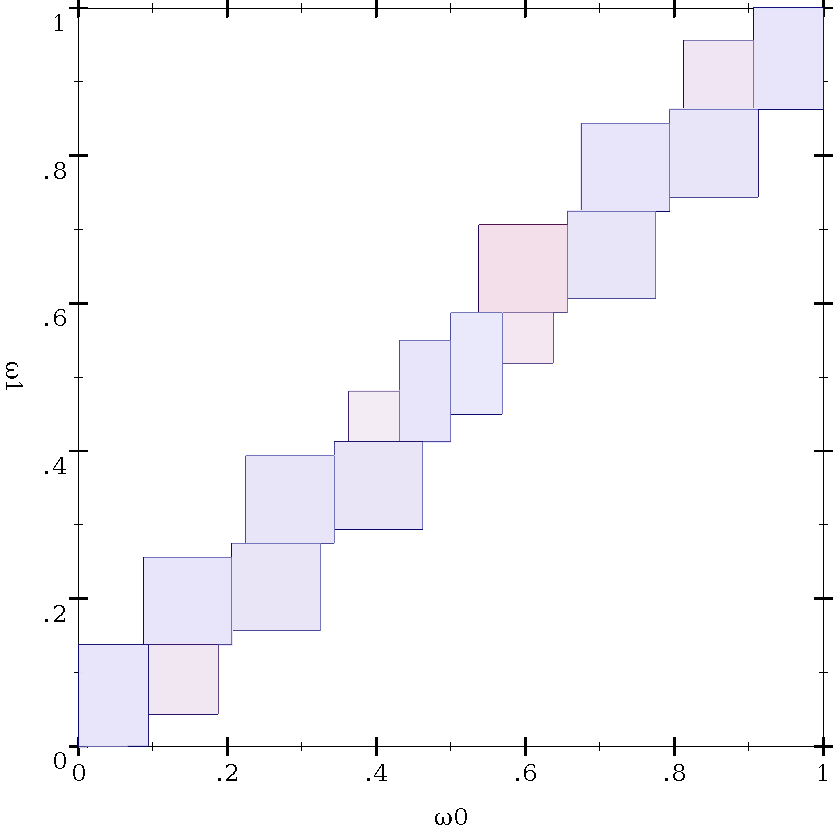
\includegraphics[width=\subfigurewidth]{results/uniform-sample-source-rects}%
\tab\tab%
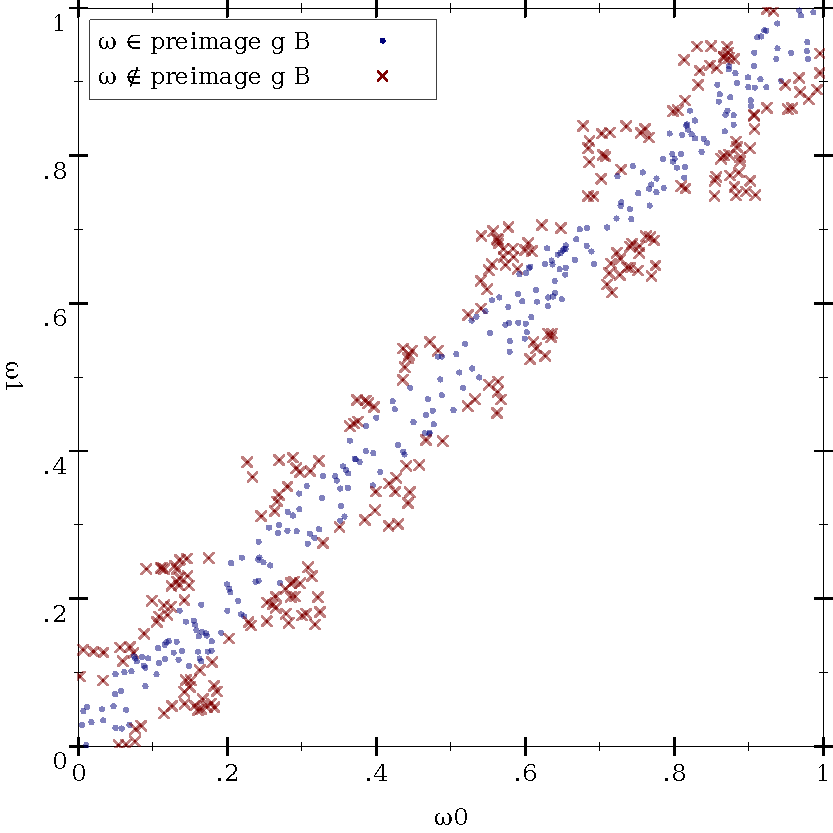
\includegraphics[width=\subfigurewidth]{results/uniform-sample-source-points}%
\end{minipage}%
}%

\subfloat[Results of $sample!part$ and $sample!source$ for the preimage of {$[-0.002,0.002]$}. Samples accepted: $30$.]{%
\label{fig:sample-source:uniform2}%
\begin{minipage}{0.98\textwidth}\centering%
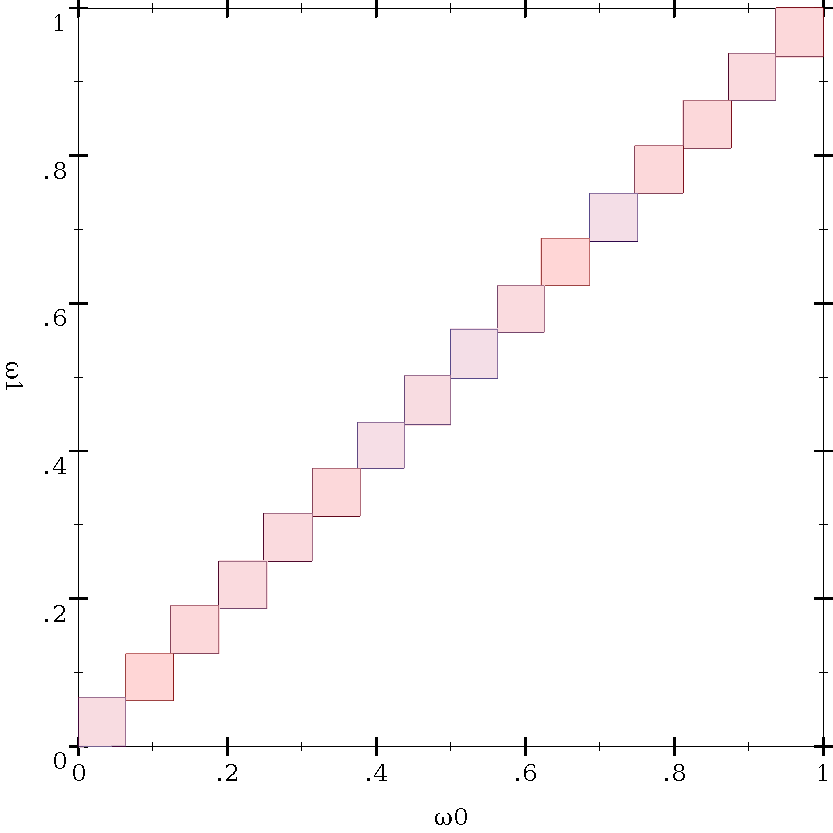
\includegraphics[width=\subfigurewidth]{results/uniform-sample-source-rects2}%
\tab\tab%
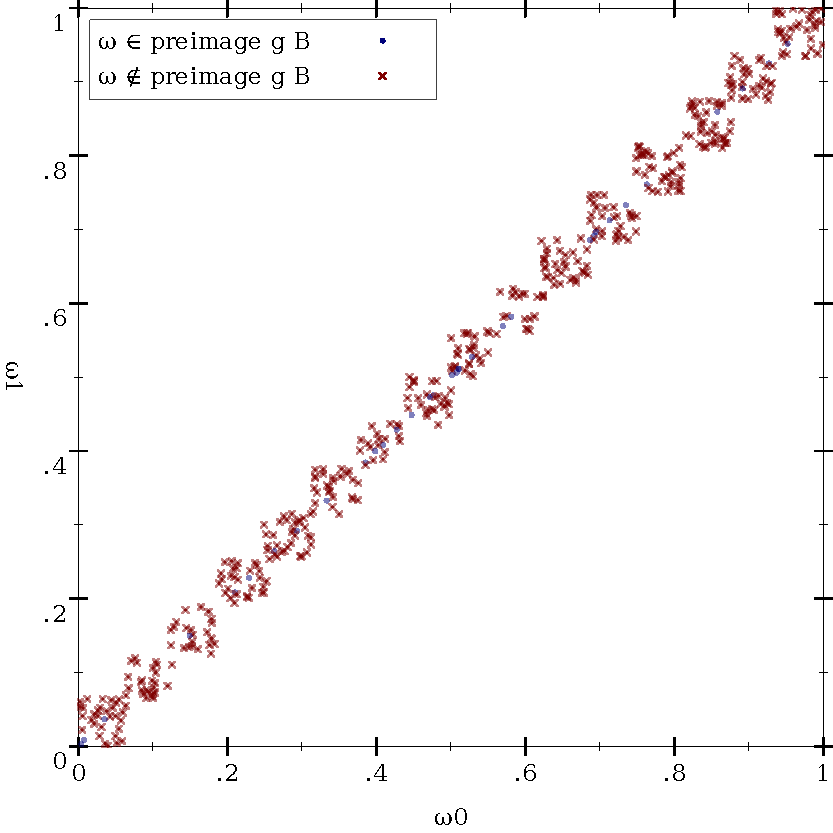
\includegraphics[width=\subfigurewidth]{results/uniform-sample-source-points2}%
\end{minipage}%
}%

\subfloat[Results of $sample!part$ and $sample!source^*$ for the preimage of {$[-0.002,0.002]$}. Samples accepted: $500$.]{%
\label{fig:sample-source:nonuniform}%
\begin{minipage}{0.98\textwidth}\centering%
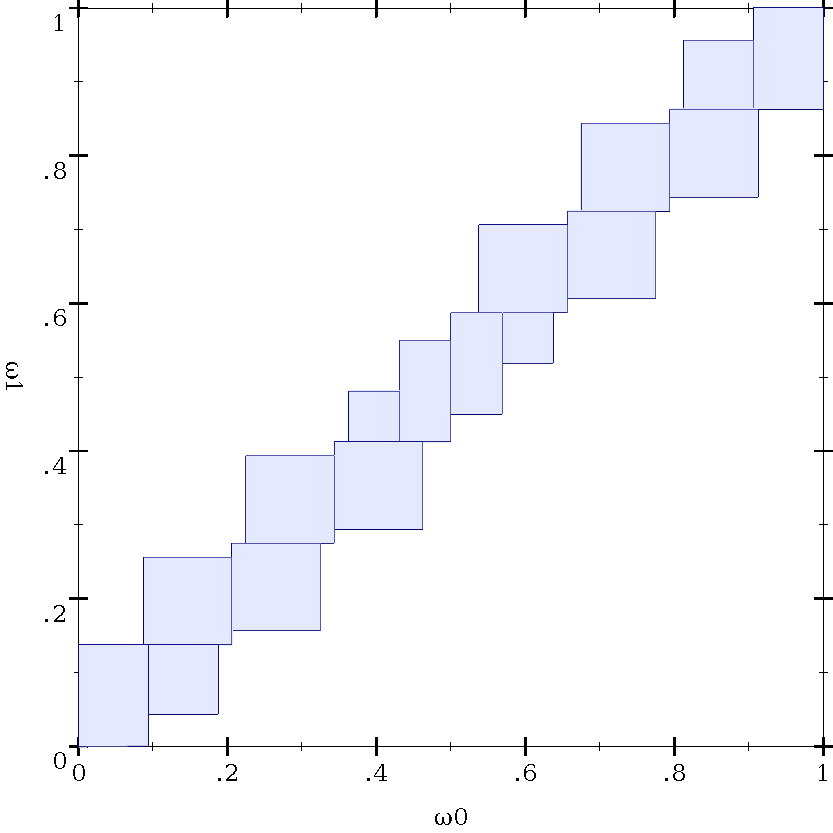
\includegraphics[width=\subfigurewidth]{results/nonuniform-sample-source-rects}%
\tab\tab%
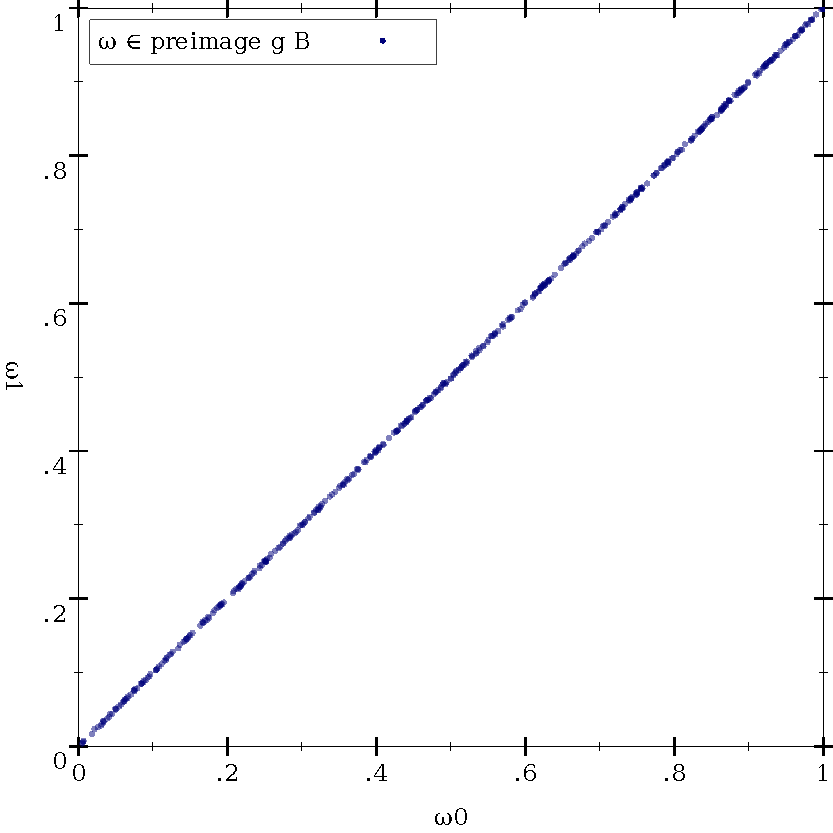
\includegraphics[width=\subfigurewidth]{results/nonuniform-sample-source-points}%
\end{minipage}%
}
\caption[]{$500$ samples using Dr. Bayes's implementations of $sample!part$, $sample!source$ and $sample!source^*$.}
\label{fig:sample-source}
\end{figure*}


Figure~\ref{fig:sample-source:uniform} shows the result of sampling within the preimage of $[-0.05,0.05]$ under the interpretation of this program as a random variable:
\begin{center}\singlespacing
\begin{schemedisplay}
(define/drbayes diagonal
  (let ([x  (random)]
        [y  (random)])
    (- y x)))
\end{schemedisplay}
\end{center}
The left plot shows the results returned by the implementation of $sample!part$: sampled parts from a rectangle covering the true preimage, which surrounds the line $\omega_1 = \omega_0$.
(There are many duplicates.)
The right plot shows the result of sampling once within each part uniformly; in this case, 244 out of 500 samples are inside the preimage set.

Figure~\ref{fig:sample-source:uniform2} shows the result of sampling within the preimage of $[-0.002,0.002]$, for which many fewer samples are in the preimage set; in this case, only 30.
In general, for the interpretation of \scheme{diagonal}, the proportion of accepted samples in the preimage of $[-\epsilon,\epsilon]$ scales linearly with $\epsilon$.
We can mitigate this problem using finer partitions of $proj~j~\Omega'$.
However, there is a solution that does not require finer partitions and accepts more samples than any repartitioning.

The key insight is that the singleton interval $\set{b} = [b,b]$ is also a rectangle.
To sample within a part, for each axis $j \in J'$, we choose $b \in proj~j~\Omega'$, update $\Omega'$ using $unproj~j~\Omega'~\set{b}$, and use $refine$ to get better bounds for sampling the other axes.

The following function implements the idea.
\begin{equation}
\begin{aligned}
	&sample!source^* : [J] \tto \pair{\Re,Rect~\pair{\Omega, T}} \tto \pair{\Re,\Omega_\bot} \\
	&\lzfcsplit[@{}l@{}l@{}]{
	&sample!source^*~js~\pair{q_\omega,\emptyset} &\ :=\ \pair{0,\bot} \\
	&sample!source^*~\pair{}~\pair{q_\omega,\Omega' \times T'}&\ :=\ 
		\lzfclet{
			\omega & \fun{j \in J} sample!uniform~(proj~j~\Omega')
		}{\pair{q_\omega, \omega}}
\\
	&sample!source^*~\pair{j,js}~\pair{q_\omega,\Omega' \times T'}&\ :=\ 
		\lzfclet{
			B & proj~j~\Omega' \\
			b & sample!uniform~B \\
			A' & refine~(unproj~j~\Omega'~\set{b} \times T')
		}{sample!source^*~js~\pair{q_\omega \cdot 1{/}(m~B),A'}}
	}
\end{aligned}
\label{eqn:sample-source*}
\end{equation}
Here, $[J]$ is the type of lists of $J$, or $\pair{J,\pair{J,... \pair{J,\pair{}}}}$.
The caller is expected to linearize $J'$, the indexes of random values that are actually used while running the program, as $js : [J]$.
(Dr. Bayes's implementation of $sample!part$ returns $js$ in addition to the covering rectangle and its probability.)
The density of the sampled $\omega$ is computed as $\prod_{j \in J'} 1{/}(m~(proj~j~\Omega'_j))$, where $\Omega'_j$ are the ever-shrinking inputs to $sample!source^*$.
Roughly, it is the joint density of \emph{dependent} uniform random variables evaluated at $restrict~\omega~J'$.

Figure~\ref{fig:sample-source:nonuniform} shows the result of using Dr. Bayes's implementation of $sample!source^*$ to sample within parts.
No samples are rejected: in all cases, choosing an $\omega_0$ and updating $\Omega'$ with $\set{\omega_0}$ allows preimage refinement to determine the range of values for $\omega_1$ for which $\omega$ is in the preimage set.

Samples taken using $sample!source^*$ may still be rejected, when sampling from an overapproximated projection causes $refine$ to return $\emptyset$.
We demonstrate and characterize the conditions under which this happens in Chapter~\ref{ch:examples}.

\subsection{Self-Adjusting Probabilistic Search}
\label{sec:self-adjusting}

One way to regard $sample!part$ is as a search for nonempty sets.

To be correct, $sample!part$ must return the actual probabilities with which it chooses each rectangular part cover.
The easiest way to do so is to ensure that the transformation from random choices to part covers is injective: that no two combinations of choices result in the same part cover.
Then the part cover's probability is the product of the choice probabilities.

This unfortunately rules out backtracking search, because many backtracking paths can result in the same rectangular cover.
Fortunately, because we invoke $sample!part$ many times, past results can inform future ones.

The main idea is this: instead of just searching by making random choices, build a tree of possible searches.
Each child node represents a choice, and parents label their children with probabilities.
Leaf nodes contain rectangular part covers.
To choose a part cover, repeatedly choose child nodes according to their probabilities.
If the resulting leaf's cover is $\emptyset$, remove it from the tree and adjust the child probabilities.
Thus, choice combinations that lead to failure occur at most once.
If child probabilities are correctly adjusted, removing a failure leaf does not change the probabilities of successful ones.

\begin{figure*}[tb!]\centering%
\subfloat[A random path leading to a failure leaf]{%
\label{fig:self-adjusting-search-tree:fail}%
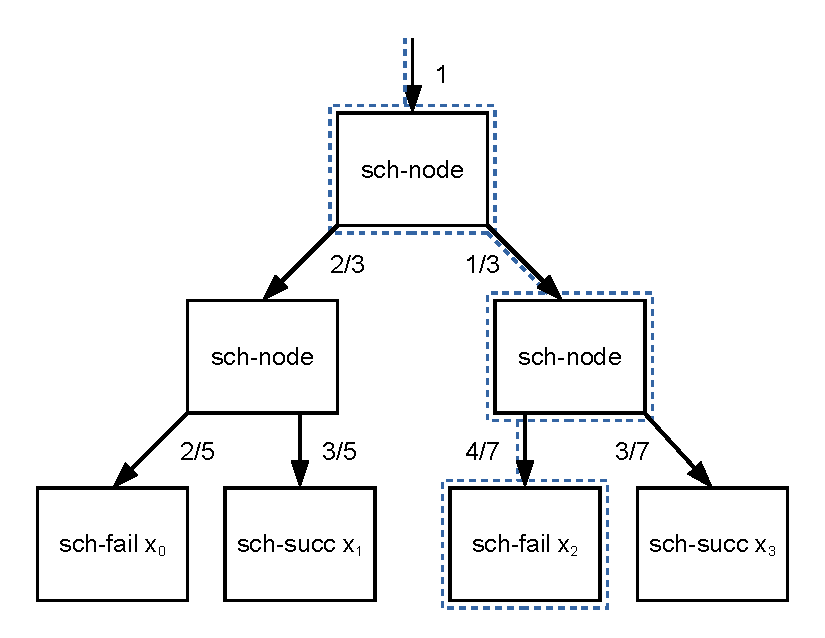
\includegraphics[width=3.4375in]{figures/search-tree-1}%
}%
\tab%
\subfloat[An adjusted tree with $x_2$ removed]{%
\label{fig:self-adjusting-search-tree:adjusted}%
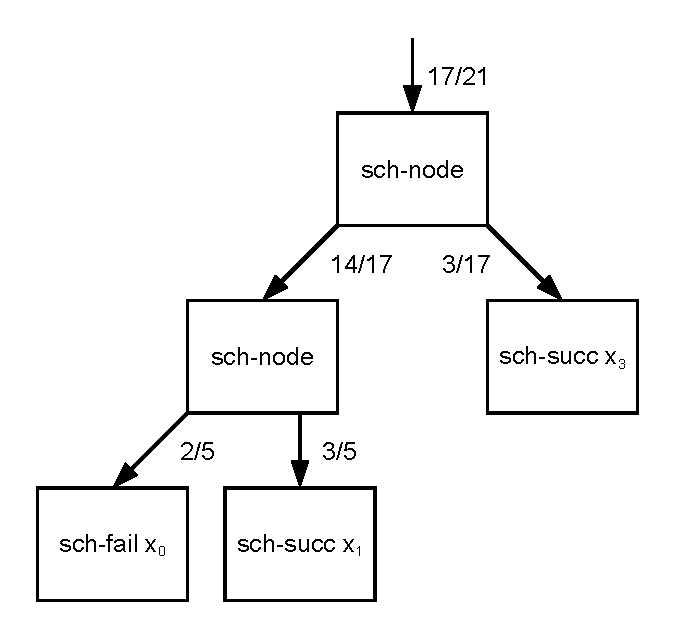
\includegraphics[width=2.8125in]{figures/search-tree-2}%
}
\caption[Self-adjusting, probabilistic tree search]{A self-adjusting, probabilistic tree search. After $sch!fail~x_2$ is discovered to be a failure node, the path to the root is updated to remove it and maintain the probabilities of the other leaves.}
\label{fig:self-adjusting-search-tree}
\end{figure*}

Figure~\ref{fig:self-adjusting-search-tree:fail} illustrates the self-adjusting search more generally.
Four boxes represent two failure leaves with values $x_0$ and $x_2$, and two success leaves with values $x_1$ and $x_3$.
Each leaf value is distinct.
Each node has two children, each with some probability, and the child probabilities sum to $1$.
The dotted outlines show a random path down the search tree ending on a failure leaf $x_2$.
The probability of this failure is $1 \cdot 1{/}3 \cdot 4{/}7 = 4{/}21$.

To remove it, we must update the entire path back up to the root in a way that maintains the probabilities of every other leaf.
Figure~\ref{fig:self-adjusting-search-tree:adjusted} shows the result of having done so.
For example, the probability of $x_3$ is $1 \cdot 1{/}3 \cdot 3{/}7 = 1{/}7$ in the original tree, and is still $17{/}21 \cdot 3{/}17 = 1{/}7$ in the adjusted tree.

\begin{figure*}[!tb]\centering
\smallmathfont
\begin{align*}
\begin{aligned}[t]
	&\begin{aligned}[t]
		Search~X\ ::=
			&\ sch!fail~X \\
			|&\ sch!succ~X \\
			|&\ sch!node~\pair{(0,1],Search~X}~\pair{(0,1],Search~X}
	\end{aligned} \\
\\[-6pt]
	&\begin{aligned}[t]
		&adjusted!node : (0,1] \tto \pair{[0,1],Search~X} \tto \pair{(0,1],Search~X} \tto \pair{(0,1],Search~X} \\
		&\lzfcsplit[@{}l@{}l@{}]{
			&adjusted!node~p_t~\pair{0,\uscore}~\pair{p_r,c_r} &\ :=\ \pair{p_t \cdot p_r,c_r} \\
			&adjusted!node~p_t~\pair{p_l,c_l}~\pair{p_r,c_r} &\ :=\ 
				\lzfclet{
					p_{lr} & p_l + p_r
				}{\pair{p_t \cdot p_{lr}, sch!node~\pair{p_l{/}p_{lr}, c_l}~\pair{p_r{/}p_{lr}, c_r}}}
		}
	\end{aligned} \\
\\[-6pt]
	&\begin{aligned}[t]
		&sample!search : \pair{(0,1],Search~X} \tto \pair{\pair{(0,1],X},\pair{[0,1],Search~X}} \\
		&\lzfcsplit[@{}l@{}l@{}]{
			&sample!search~\pair{p_x,sch!succ~x} &\ :=\ \pair{\pair{p_x,x},\pair{p_x,sch!succ~x}} \\
			&sample!search~\pair{p_x,sch!fail~x} &\ :=\ \pair{\pair{p_x,x},\pair{0,sch!fail~x}} \\
			&sample!search~\pair{p_t,sch!node~l~r} &\ :=\ 
				\lzfclet{
					sch!node~\pair{p_l,c_l}~r' &
						if~\lzfcsplit{
							&(sample!bool~(fst~l)) \\
							&(sch!node~l~r) \\
							&(sch!node~r~l)
						} \\
					\pair{px,\pair{p_t',c_l'}} & sample!search~\pair{p_t \cdot p_l, c_l} \\
					p_l' & p_t'{/}p_t
				}{\pair{px,adjusted!node~p_t~\pair{p_l',c_l'}~r'}}
		}
	\end{aligned}
\end{aligned}
\end{align*}
\bottomhrule
\caption[Self-adjusting, probabilistic tree search algorithm]{A data type and algorithm for a self-adjusting, probabilistic tree search.}
\label{fig:self-adjusting-search}
\end{figure*}

Figure~\ref{fig:self-adjusting-search} defines $Search~X$, the type of search trees with leaf values $X$.
To keep the presentation simple, values with type $Search~X$ are finite trees.
It is easy to extend it to include lazy trees, and not much harder to change $sample!part$ to build and update an instance of $\pair{\Re,Search~(Rect~\pair{\Omega,T})}$ instead of sampling directly.
From here on, we consider only trees in which every pair of child probabilities sums to $1$ and every leaf value in the tree is unique.

The $sample!search$ function carries out the self-adjusting probabilistic search.
It receives a probability and a $Search~X$ instance; for example, searching the tree in Figure~\ref{fig:self-adjusting-search-tree:adjusted} is done by $sample!search~\pair{17{/}21,sch!node~...}$.
It returns two pairs: $\pair{p_x,x}$, which is the sampled value and its probability, and $\pair{p_t',t'}$, which is the new search tree and its new probability.

We must be sure that $p_x$ is the probability of $x$.

\begin{theorem}[$sample!search$ returns correct probabilities]
Let $\pair{p_t,t} : \pair{\Re,Search~X}$.
Let $\pair{\pair{p_x,x},\uscore} := sample!search~\pair{p_t,t}$.
If the probability of $t$ is $p_t$, the probability of $x$ is $p_x$.
\end{theorem}
\begin{proof}
By induction on $t$. Base cases $t = sch!succ~x$ and $t = sch!fail~x$ follow directly from uniqueness of $x$.
For the inductive case $t = sch!node~\pair{p_l,c_l}~\pair{p_r,c_r}$, let $sch!node~\pair{p,c}~r' := if~(sample!bool~p_l)~...$ as in $sample!search$.
Because $p_l + p_r = 1$, $\Pspec{c = c_l} = p_t \cdot p_l$ and $\Pspec{c = c_r} = p_t \cdot p_r$.
Apply the inductive hypothesis for cases $c = c_l$ and $c = c_r$.
\end{proof}

When $sample!search$ rebuilds the path from the leaf to the root using $adjusted!node$, we must be sure that $adjusted!node$ labels the left and right children with the correct probabilities.

\begin{theorem}[$adjusted!node$ returns correct probabilities]
\label{thm:adjusted-node-correct}
Let $p_t \in (0,1]$ and $\pair{p_t',t'} := adjusted!node~p_t~\pair{p_l,c_l}~\pair{p_r,c_r}$.

If $t' = c_r$, then $p_t' = p_t \cdot p_r$.

If $t' = sch!node~\pair{p_l',c_l}~\pair{p_r',c_r}$, then $p_t' \cdot p_l' = p_t \cdot p_l$ and $p_r' \cdot p_t' = p_t \cdot p_r$.
\end{theorem}
\begin{proof}
Case $t' = c_r$. Then $p_t' = p_t \cdot p_r$ by definition of $adjusted!node$.

Case $t' = sch!node~\pair{p_l',c_l}~\pair{p_r',c_r}$.
Let $p_{lr} := p_l + p_r$, so $p_t' \cdot p_l' = (p_t \cdot p_{lr}) \cdot (p_l {/} p_{lr}) = p_t \cdot p_l$ by the definition of $adjusted!node$, and similarly for $p_t' \cdot p_r'$.
\end{proof}

Thus, using $adjusted!node~p_t~\pair{p_l',c_l'}~\pair{p_r,c_r}$ to replace child $c_l$ with $c_l'$ does not affect the probabilities of leaves below $c_r$.
Further, suppose $\pair{px,\pair{p_t',c_l'}} = sample!search~\pair{p_t \cdot p_l,c_l}$ and $p_l' = p_t'{/}p_t$ as in $sample!search$.
By Theorem~\ref{thm:adjusted-node-correct}, $c_l'$ will be chosen with probability $p_l' \cdot p_t = p_t'$, as desired.

A simple extension makes trees converge not just to trees without failures, but to trees with stated probabilities for each leaf.
Consider the base cases in $sample!search$'s definition:
\begin{equation}
\begin{aligned}
	&sample!search~\pair{p_x,sch!succ~x}&&\!\! :=\ \pair{\pair{p_x,x},\pair{p_x,sch!succ~x}} \\
	&sample!search~\pair{p_x,sch!fail~x}&&\!\! :=\ \pair{\pair{p_x,x},\pair{0,sch!fail~x}} \\
\end{aligned}
\end{equation}
In both cases, returning $\pair{p,t}$ in the second of the pair causes the tree to be rebuilt so that $x$'s probability becomes $p$.
Now define, instead of $sch!succ,sch!fail : X \tto Search~X$, a constructor $sch!leaf : [0,1] \tto X \tto Search~X$ and
\begin{equation}
\begin{aligned}
	sample!search~\pair{p_x,sch!leaf~p~x}&&\!\! :=\ \pair{\pair{p_x,x},\pair{p,sch!leaf~p~x}} \\
\end{aligned}
\end{equation}
Suppose $t := sch!leaf~p_0~x_0$ is a leaf in the tree.
Sampling the initial search tree returns $x_0$ with some probability $p_x$ that is determined by the path to $t$.
With every subsequent tree after $x_0$ is first returned, sampling returns $x_0$ with probability $p_0$.

A version of $sample!part$ that builds such trees using $sch!leaf$ might use the actual measure of the part cover $\Omega'$ as its probability.
Recall, however, that partitioned importance sampling requires $sample!part$ to choose parts according to a fixed probability measure.
We are fairly certain that partitioned importance sampling is correct even when the distribution over parts varies, as long as it converges pointwise, but we have not yet proved it.

\section{Conclusions}

\begin{figure*}[tb!]\centering
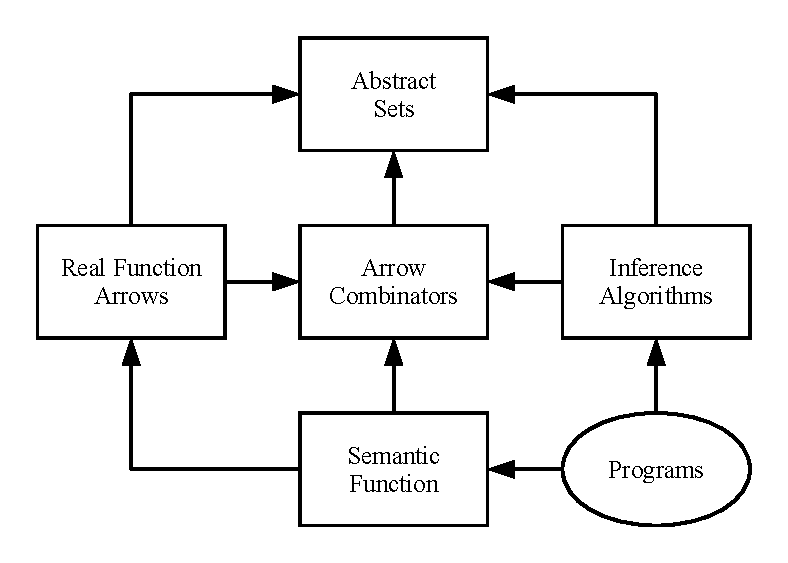
\includegraphics[width=4.75in]{figures/implementation-components-2}
\caption[Implementation dependency graph]{The implementation components that make up Dr. Bayes and their dependence structure.}
\label{fig:implementation-components-2}
\end{figure*}

Figure~\ref{fig:implementation-components-2} again shows the components in the implementation of Dr. Bayes.

Chapter~\ref{ch:preimage1} defined the semantic function that transforms programs into their meanings.
It derived the approximating preimage* arrow and proved it terminating and correct, provided representations of abstract sets and operations on them are correct, as well as any lifts of primitive functions.

In this chapter, we detailed the implementation of a simple abstract set library.
Many of its functions are derived from lattice and set properties.
We additionally verified through randomized testing that 21 sufficient lattice and membership properties hold.

We began a general theory of approximate function inversion, and used it to derive correct computations of preimages under one-argument, real bijections such as square roots, and two-argument trijections such as addition on $\Re \times \Re$ and multiplication on open quadrants.
The theory allows simultaneous implementation for functions related by inversion and axial inversion.
More complicated functions are built from simpler pieces using arrow combinators.

We developed a partitioned importance sampling algorithm and proved that it preserves expected values.
We proved that our implementation of it is correct and terminates, and developed extensions that reduce the rejection rate of sampling within a part, and allow part sampling to avoid reaching $\emptyset$ the same way twice.

With Dr. Bayes implemented and verified, it is time to try programming in it.

\mathversion{normal}
